\documentclass{article}

\usepackage{arxiv}

\usepackage[utf8]{inputenc} % allow utf-8 input
\usepackage[T1]{fontenc}    % use 8-bit T1 fonts
\usepackage{lmodern}        % https://github.com/rstudio/rticles/issues/343
\usepackage{hyperref}       % hyperlinks
\usepackage{url}            % simple URL typesetting
\usepackage{booktabs}       % professional-quality tables
\usepackage{amsfonts}       % blackboard math symbols
\usepackage{nicefrac}       % compact symbols for 1/2, etc.
\usepackage{microtype}      % microtypography
\usepackage{graphicx}

\title{A Statistical Perspective of Non-Inferiority Trials}

\author{
    Áine Glynn
   \\
    University of Galway \\
   \\
  \texttt{} \\
   \And
    Filip Kłosowski
   \\
    University of Galway \\
   \\
  \texttt{} \\
  }


% tightlist command for lists without linebreak
\providecommand{\tightlist}{%
  \setlength{\itemsep}{0pt}\setlength{\parskip}{0pt}}


% Pandoc citation processing
%From Pandoc 3.1.8
% definitions for citeproc citations
\NewDocumentCommand\citeproctext{}{}
\NewDocumentCommand\citeproc{mm}{%
  \begingroup\def\citeproctext{#2}\cite{#1}\endgroup}
\makeatletter
 % allow citations to break across lines
 \let\@cite@ofmt\@firstofone
 % avoid brackets around text for \cite:
 \def\@biblabel#1{}
 \def\@cite#1#2{{#1\if@tempswa , #2\fi}}
\makeatother
\newlength{\cslhangindent}
\setlength{\cslhangindent}{1.5em}
\newlength{\csllabelwidth}
\setlength{\csllabelwidth}{3em}
\newenvironment{CSLReferences}[2] % #1 hanging-indent, #2 entry-spacing
 {\begin{list}{}{%
  \setlength{\itemindent}{0pt}
  \setlength{\leftmargin}{0pt}
  \setlength{\parsep}{0pt}
  % turn on hanging indent if param 1 is 1
  \ifodd #1
   \setlength{\leftmargin}{\cslhangindent}
   \setlength{\itemindent}{-1\cslhangindent}
  \fi
  % set entry spacing
  \setlength{\itemsep}{#2\baselineskip}}}
 {\end{list}}
\usepackage{calc}
\newcommand{\CSLBlock}[1]{#1\hfill\break}
\newcommand{\CSLLeftMargin}[1]{\parbox[t]{\csllabelwidth}{#1}}
\newcommand{\CSLRightInline}[1]{\parbox[t]{\linewidth - \csllabelwidth}{#1}\break}
\newcommand{\CSLIndent}[1]{\hspace{\cslhangindent}#1}

\usepackage{fontspec}
\usepackage{float}
\usepackage{amsmath}
\usepackage{amssymb}
\usepackage{bm}
\usepackage{booktabs}
\usepackage{graphicx}
\usepackage{array}
\usepackage[table]{xcolor}
\usepackage{geometry}
\usepackage{setspace}
\usepackage{caption}
\usepackage{subcaption}
\usepackage{placeins}
\setlength{\textfloatsep}{6pt plus 2pt minus 2pt}
\setlength{\floatsep}{6pt plus 2pt minus 2pt}
\setlength{\intextsep}{6pt plus 2pt minus 2pt}
\setlength{\abovecaptionskip}{3pt}
\setlength{\belowcaptionskip}{3pt}
\usepackage{hyperref}
\hypersetup{colorlinks=true, linkcolor=black, citecolor=black, urlcolor=blue, filecolor=black}
\usepackage{tocloft}
\let\oldmaketitle\maketitle
\renewcommand{\maketitle}{\begin{center}
\includegraphics[width=4cm]{Figures/logo2UG.png}\end{center}\vspace{0.5cm}\oldmaketitle}
\begin{document}
\maketitle


\begin{abstract}
Single-arm performance goal studies are widely used in medical device
evaluation when a randomised active-control trial is impractical or
ethically unjustifiable. The trial conclusion depends on whether a
pre-specified performance goal is met, as determined by a hypothesis
test or confidence interval procedure applied to the observed outcome.
Despite their apparent simplicity, the conclusions of such studies are
sensitive to three interconnected methodological choices: the derivation
and value of the performance goal, the confidence interval method used
to construct the decision rule and the assumptions underlying the sample
size calculation. This thesis examines each of these choices in the
context of a retrospective case study of a vascular stent developed for
the treatment of femoropopliteal peripheral artery disease.

Performance goals for a 30-day composite safety endpoint and a 12-month
Rutherford classification efficacy endpoint were derived through a
meta-analysis of three historical femoropopliteal bare nitinol stent
studies comprising 116 patients. Confidence interval boundaries rather
than point estimates were proposed to account for uncertainty in the
historical evidence, yielding a maximum acceptable 30-day composite
adverse event proportion of 12\% and a minimum acceptable 12-month
Rutherford success proportion of 88\%. The limited evidence base
produced wide uncertainty around both estimates, illustrating that
performance goals carry inherent uncertainty that is not always evident
when they are reported as fixed values.

A simulation study evaluated six confidence interval methods for binary
proportions across a grid of true event proportions and sample sizes
relevant to case study endpoints that lie near the margins of a
probabilistic range (e.g.~near zero). The Wald consistently fell below
the nominal 95\% coverage level making it unsuitable for this setting.
Among the remaining methods, Wilson Score and Jeffreys achieved coverage
closest to the nominal level with the relatively narrow intervals, while
Clopper-Pearson, Agresti-Coull and the continuity-corrected Wilson Score
were conservative with progressively wider intervals. These differences
in coverage behaviour translated into meaningful differences in sample
size requirements. Under an approved performance goal of 11\%, an
assumed true complication proportion of 5\% and a target power of 90\%,
Clopper-Pearson was used as the primary method, requiring 209 evaluable
patients at 89.7\% achieved power. Among methods meeting the nominal
coverage level, the required sample size ranged from 198 patients under
Jeffreys to 247 patients under the continuity-corrected Wilson Score.

An interactive R Shiny application, PG-Power, was developed to implement
the proposed sample size framework and provide a transparent, accessible
and reproducible assessment of the sensitivity of required sample sizes
to different design assumptions. The application supports confidence
interval method comparison, power curve visualisation, sensitivity
analysis and report generation for single-arm performance goal studies.

The thesis concludes with an exploration of Bayesian historical
borrowing as a framework for formally incorporating prior evidence into
the sample size calculation, under the assumption that historical and
current patient populations are sufficiently exchangeable to justify
combining information across studies.

The findings demonstrate that the performance goal value, confidence
interval method and assumptions underlying the sample size calculation
each can alter the design requirements and the conclusion of a
performance goal study independently of the underlying clinical data.
Transparent derivation and pre-specification of these choices in the SAP
is essential to the credibility and reproducibility of performance goal
studies in medical device evaluation.
\end{abstract}

\keywords{
    Binomial confidence intervals
   \and
    Performance goals
   \and
    Single-arm clinical trials
   \and
    Medical device evaluation
   \and
    Sample size calculation
   \and
    Bayesian historical borrowing
  }

\newpage

\section*{Acknowledgments}\label{acknowledgments}
\addcontentsline{toc}{section}{Acknowledgments}

We would like to sincerely thank Prof.~John Newell for his guidance,
encouragement and support throughout this project. His expertise and
passion for his field, combined with his consistent energy, welcoming
nature and humour made this experience both memorable and inspiring. We
are also grateful to the lead scientist involved in the BioMimics 3D
trial for sharing their time, experience and insight with us. Our
meetings provided a valuable opportunity to understand the journey of a
clinical trial from a statistical and practical perspective. Both
experiences provided us with a glimpse into the work we hope to
contribute to in our future careers.

\newpage
\tableofcontents
\newpage
\listoffigures
\listoftables
\newpage

\section*{Abbreviations and Acronyms}\label{abbreviations-and-acronyms}
\addcontentsline{toc}{section}{Abbreviations and Acronyms}

\begin{tabular}{ll}
SAP & Statistical Analysis Plan \\
TVR & Target Vessel Revascularisation \\
PAD & Peripheral Artery Disease \\
ESS & Effective Sample Size \\
\end{tabular}

\newpage

\section{Introduction}\label{introduction}

\subsection{Single Arm Non-inferiority
Trials}\label{single-arm-non-inferiority-trials}

Single Arm non-inferiority trials arise when an effective treatment or
device already exists and a placebo-controlled comparison would be
unethical, impractical or clinically uninformative
(\citeproc{ref-schumi_through_2011}{1}--\citeproc{ref-oczkowski_clinicians_2014}{3}).
Rather than demonstrating superiority, the goal is to show that any loss
of efficacy associated with the new intervention remains within a
clinically acceptable limit
(\citeproc{ref-schumi_through_2011}{1}--\citeproc{ref-oczkowski_clinicians_2014}{3}).
This limit, known as the non-inferiority margin, represents the largest
reduction in efficacy considered tolerable in exchange for other
benefits such as improved safety, simpler delivery, lower cost or better
patient adherence
(\citeproc{ref-schumi_through_2011}{1},\citeproc{ref-cuzick_interpreting_2022}{2},\citeproc{ref-tweed_exploring_2024}{4}).

The trial conclusion depends on both the observed treatment effect and
the uncertainty surrounding it
(\citeproc{ref-schumi_through_2011}{1},\citeproc{ref-cuzick_interpreting_2022}{2},\citeproc{ref-international_council_for_harmonisation_statistical_1998}{5}).
In practice, this uncertainty is assessed by comparing a confidence
interval for the treatment effect against the pre-specified
non-inferioirty margin
(\citeproc{ref-schumi_through_2011}{1},\citeproc{ref-cuzick_interpreting_2022}{2},\citeproc{ref-piaggio_reporting_2012}{6}).
For favourable endpoints, where higher values indicate better
performance, the lower confidence bound is the relevant measure, while
for unfavourable endpoints the upper bound is used
(\citeproc{ref-schumi_through_2011}{1},\citeproc{ref-cuzick_interpreting_2022}{2}).
This one-sided structure distinguishes non-inferiority trials from
superiority and equivalence designs, and places the choice of margin and
confidence interval method at the centre of the trial's interpretation
(\citeproc{ref-schumi_through_2011}{1}--\citeproc{ref-oczkowski_clinicians_2014}{3},\citeproc{ref-piaggio_reporting_2012}{6}).

\subsection{Performance Goals in Medical Device
Studies}\label{performance-goals-in-medical-device-studies}

Performance goal studies are similar to single-arm non-inferiority
designs and are particularly common in medical device trials
(\citeproc{ref-schumi_through_2011}{1},\citeproc{ref-wang_leveraging_2021}{7},\citeproc{ref-wang_single-arm_2024}{8}).
Rather than comparing the observed outcome against a non-inferiority
margin derived from a comparator treatment, performance goal studies
compare the observed outcome with a pre-specified benchmark derived from
historical evidence and clinical judgement
(\citeproc{ref-wang_leveraging_2021}{7},\citeproc{ref-rocha-singh_performance_2007}{9}).
This benchmark defines the acceptable level of performance for the
device under evaluation, representing either a minimum acceptable
proportion for favourable (efficacy) endpoints or a maximum acceptable
proportion for unfavourable (safety) endpoints.
(\citeproc{ref-wang_leveraging_2021}{7},\citeproc{ref-rocha-singh_performance_2007}{9}).

Preformance goal studies are useful when a randomised active-control
trial is difficult to justify or conduct
(\citeproc{ref-wang_leveraging_2021}{7},\citeproc{ref-wang_single-arm_2024}{8}).
However, the absence of a concurrent comparator makes the choice of
benchmark especially consequential
(\citeproc{ref-wang_leveraging_2021}{7},\citeproc{ref-cao_estimating_2025}{10}).
Historical studies may differ from the current trial in ways that affect
the validity of the comparison, including differences in the target
population, endpoint definitions, follow-up duration and broader
clinical practice
(\citeproc{ref-wang_leveraging_2021}{7},\citeproc{ref-cao_estimating_2025}{10}).
These differences must be carefully considered when constructing and
justifying a performance goal.

The direction of the performance goal depends on the nature of the
endpoint
(\citeproc{ref-wang_leveraging_2021}{7},\citeproc{ref-rocha-singh_performance_2007}{9}).
For efficacy endpoints, where higher event proportions reflect better
performance, the estimated proportion and its confidence interval must
exceed a predefined minimum acceptable level
(\citeproc{ref-wang_leveraging_2021}{7},\citeproc{ref-rocha-singh_performance_2007}{9}).
For safety endpoints, where lower proportions are desirable, the
estimated proportion and its confidence interval must remain below a
predefined maximum acceptable level of harm
(\citeproc{ref-wang_leveraging_2021}{7},\citeproc{ref-rocha-singh_performance_2007}{9}).
In either case, a performance goal should not be treated as a simple
numerical cut-off
(\citeproc{ref-international_council_for_harmonisation_statistical_1998}{5},\citeproc{ref-wang_leveraging_2021}{7},\citeproc{ref-rocha-singh_performance_2007}{9}).
It represents a clinical and statistical threshold whose validity
depends on the endpoint being measured, the quality and consistency of
the historical evidence, and the level of uncertainty considered
acceptable for regulatory decision-making
(\citeproc{ref-wang_leveraging_2021}{7},\citeproc{ref-wang_single-arm_2024}{8},\citeproc{ref-cao_estimating_2025}{10}).

\subsection{Motivation for Study}\label{motivation-for-study}

Although non-inferiority and performance goal designs appear
straightforward in principle, their conclusions can be sensitive to
several methodological choices
(\citeproc{ref-schumi_through_2011}{1}--\citeproc{ref-oczkowski_clinicians_2014}{3}).
Small variations in any of these decisions can alter the interpretation
of the same clinical data and, consequently, the study conclusion
(\citeproc{ref-schumi_through_2011}{1},\citeproc{ref-cuzick_interpreting_2022}{2}).

This sensitivity is particularly consequential in medical device
studies, where single-arm performance goal designs are common and the
absence of a concurrent comparator means the benchmark carries much of
the evidential weight
(\citeproc{ref-wang_leveraging_2021}{7},\citeproc{ref-wang_single-arm_2024}{8},\citeproc{ref-noauthor_medical_2026}{11}).
If the benchmark is too lenient, a device may appear acceptable despite
a clinically meaningful loss of performance. If it is too strict, a
device that performs well may require an impractically large sample size
or fail to meet the criterion regardless
(\citeproc{ref-tweed_exploring_2024}{4},\citeproc{ref-wang_leveraging_2021}{7},\citeproc{ref-cao_estimating_2025}{10}).
In either case, the benchmark itself shapes the conclusion before a
single patient is enrolled.

Previous reviews have raised concerns about how consistently these
choices are reported. Piaggio et al.~found that only around one-fifth of
332 non-inferiority and equivalence trials published between 1990 and
2000 provided a suitable rationale for the chosen margin
(\citeproc{ref-piaggio_reporting_2012}{6}). A later review of 232 drug
trials found that while nearly all reports specified a margin, only 24\%
explained how it had been determined
(\citeproc{ref-piaggio_reporting_2012}{6}). Together these findings
point to a recurring problem: margins and performance goals are often
presented as settled values without making the reasoning behind them
transparent
(\citeproc{ref-cuzick_interpreting_2022}{2},\citeproc{ref-piaggio_reporting_2012}{6}).

This study is motivated by that problem. Using the BioMimics 3D vascular
stent trial as a case study, it examines how performance goal selection,
confidence interval choice and the assumptions underlying the sample
size calculation interact to influence the design requirements and
conclusions in a single-arm medical device setting
(\citeproc{ref-schumi_through_2011}{1},\citeproc{ref-international_council_for_harmonisation_statistical_1998}{5},\citeproc{ref-wang_leveraging_2021}{7}).

\subsection{Case Study: BioMimics 3D Vascular
Stent}\label{case-study-biomimics-3d-vascular-stent}

The BioMimics 3D vascular stent trial serves as the primary case study
throughout this analysis. Rather than attempting to reproduce the
original trial, the case study is used as a real-world medical device
example to examine how statistical choices surrounding performance
goals, confidence intervals and sample size assumptions influence the
interpretation of device performance.

Clinical and regulatory context for the analysis was obtained through
meetings with a lead scientist involved in the original trial. These
discussions clarified how the device was intended to be evaluated in
practice and highlighted that the statistical design could not be
reduced to a purely numerical exercise --- it had to reflect clinical
judgement, regulatory expectations and practical feasibility alongside
the available evidence.

\subsection{Study Aims}\label{study-aims}

This study has five objectives:

\begin{enumerate}
\def\labelenumi{\arabic{enumi}.}
\tightlist
\item
  To derive evidence-based performance goals for a single-arm medical
  device study through meta-analysis of comparable historical device
  studies;
\item
  To compare confidence interval methods for binary endpoints in terms
  of coverage probability and interval width;
\item
  To evaluate how performance goal selection and confidence interval
  choice affect sample size requirements and non-inferiority
  conclusions;
\item
  To develop an interactive Shiny application, PG-Power, to support
  sample size planning and confidence interval method selection in
  performance goal studies;
\item
  To explore the potential role of Bayesian historical borrowing as a
  means of reducing the required sample size.
\end{enumerate}

\section{Background and Statistical
Framework}\label{background-and-statistical-framework}

\subsection{Superiority, Equivalence and
Non-Inferiority}\label{superiority-equivalence-and-non-inferiority}

Superiority, equivalence, and non-inferiority trials address distinct
clinical questions and cannot be interpreted interchangeably
(\citeproc{ref-lesaffre_superiority_2008}{12},\citeproc{ref-chow_sample_2017}{13}).
Let \(p_T\) denote the success probability in the investigational
treatment group and \(p_C\) denote the success probability in the
comparator group. For a binary success endpoint, the treatment effect is
defined as
(\citeproc{ref-chow_sample_2017}{13},\citeproc{ref-schulz_sample_2005}{14}):

\[\theta = p_T - p_C\]

A superiority trial evaluates whether the investigational treatment
performs better than the comparator. The null and alternative hypotheses
are
(\citeproc{ref-schumi_through_2011}{1},\citeproc{ref-lesaffre_superiority_2008}{12},\citeproc{ref-chow_sample_2017}{13}):

\[H_0: \theta \leq 0 \qquad H_1: \theta > 0\]

Superiority is concluded when the lower confidence bound for \(\theta\)
lies above zero (\citeproc{ref-schumi_through_2011}{1}).

An equivalence trial asks whether the difference between treatments is
small enough to be considered clinically unimportant in either
direction. Denoting the equivalence margin as \(\Delta_E\), the
hypotheses are
(\citeproc{ref-piaggio_reporting_2012}{6},\citeproc{ref-lesaffre_superiority_2008}{12},\citeproc{ref-chow_sample_2017}{13}):

\[H_0: \theta \leq -\Delta_E \text{ or } \theta \geq \Delta_E \qquad H_1: -\Delta_E < \theta < \Delta_E\]

Equivalence is concluded when the confidence interval for \(\theta\)
lies entirely within the equivalence margins
(\citeproc{ref-piaggio_reporting_2012}{6},\citeproc{ref-lesaffre_superiority_2008}{12},\citeproc{ref-chow_sample_2017}{13}):

\[-\Delta_E < \text{CI}_{1-\alpha}(\theta) < \Delta_E\]

A non-inferiority trial is less restrictive, focusing only on
differences in the unfavourable direction. Denoting the non-inferiority
margin as \(\Delta_{NI}\), the largest clinically acceptable loss of
efficacy, the hypotheses are
(\citeproc{ref-schumi_through_2011}{1},\citeproc{ref-cuzick_interpreting_2022}{2},\citeproc{ref-lesaffre_superiority_2008}{12},\citeproc{ref-chow_sample_2017}{13}):

\[H_0: \theta \leq -\Delta_E, \quad \theta \geq \Delta_E \qquad H_1: -\Delta_E < \theta < \Delta_E\]

Non-inferiority is concluded when the lower confidence bound lies above
the margin
(\citeproc{ref-schumi_through_2011}{1},\citeproc{ref-piaggio_reporting_2012}{6},\citeproc{ref-lesaffre_superiority_2008}{12},\citeproc{ref-chow_sample_2017}{13}):

\[L_{1-\alpha}(\theta) > -\Delta_{NI}\]

These three designs are often confused in practice, but the distinction
matters. Failure to demonstrate superiority does not imply equivalence
or non-inferiority --- a non-significant superiority test may simply
reflect insufficient power or imprecision rather than genuine similarity
between treatments
(\citeproc{ref-schumi_through_2011}{1},\citeproc{ref-cuzick_interpreting_2022}{2},\citeproc{ref-lesaffre_superiority_2008}{12}).
Each design therefore requires its own pre-specified margin, endpoints,
analysis population and decision rule, and conclusions should not be
switched between frameworks after the data have been collected
(\citeproc{ref-international_council_for_harmonisation_statistical_1998}{5},\citeproc{ref-piaggio_reporting_2012}{6},\citeproc{ref-chow_sample_2017}{13}).

\begin{figure}[H]

{\centering 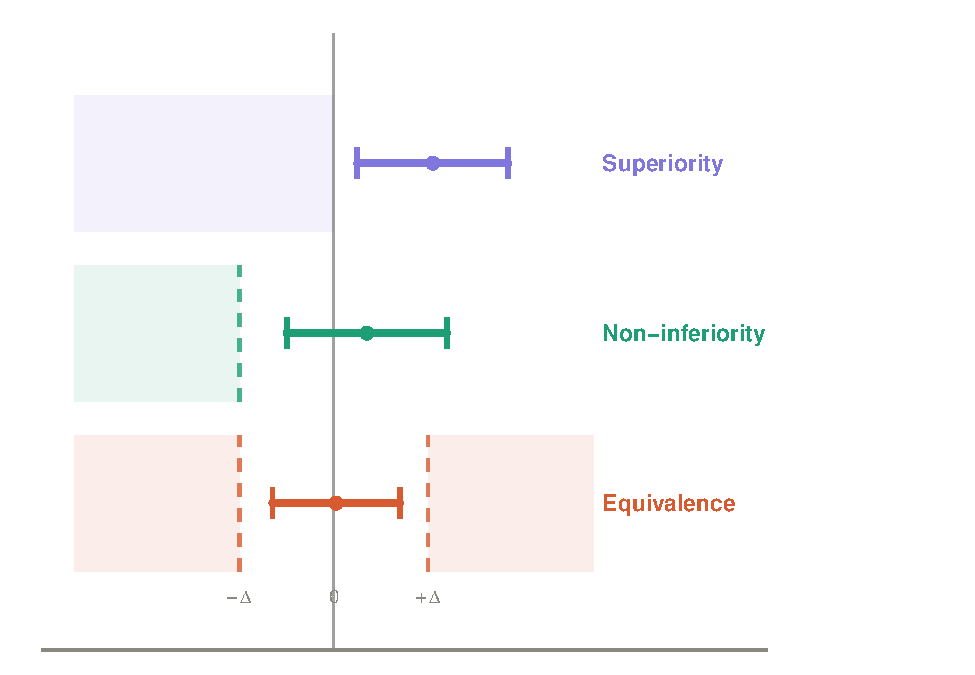
\includegraphics[width=1\linewidth]{Write_Up_Markdown_Script_files/figure-latex/trial-designs-1} 

}

\caption{Confidence interval decision rules for superiority, non-inferiority and equivalence trials. Each row shows a representative 95\% confidence interval for the treatment difference. The shaded region indicates the null hypothesis zone for each design.}\label{fig:trial-designs}
\end{figure}

\subsection{Non-Inferiority Margins and Performance
Goals}\label{non-inferiority-margins-and-performance-goals}

The non-inferiority margin is one of the central design choices in a
non-inferiority trial
(\citeproc{ref-schumi_through_2011}{1},\citeproc{ref-cuzick_interpreting_2022}{2},\citeproc{ref-us_food_and_drug_administration_non-inferiority_2016}{15}).
It defines the largest loss of efficacy considered clinically acceptable
in exchange for other benefits offered by the investigational treatment
(\citeproc{ref-schumi_through_2011}{1},\citeproc{ref-tweed_exploring_2024}{4},\citeproc{ref-us_food_and_drug_administration_non-inferiority_2016}{15}).
As established in Section 1.1, the selected margin affects the
interpretation of the trial, the required sample size and the
probability of concluding non-inferiority
(\citeproc{ref-schumi_through_2011}{1},\citeproc{ref-chow_sample_2017}{13},\citeproc{ref-us_food_and_drug_administration_non-inferiority_2016}{15}).

In an active-control non-inferiority trial, the margin is usually
defined relative to the established effect of the comparator. In
single-arm medical device studies, the same logic is applied through a
performance goal, a pre-specified benchmark against which the device is
evaluated directly, without a concurrent control group
(\citeproc{ref-wang_single-arm_2024}{8},\citeproc{ref-wang_sample_2020}{16}).
For a binary efficacy endpoint, where higher proportions reflect better
performance, the hypotheses take the form:

\[H_0: p \leq p_0 \qquad H_1: p > p_0\]

where \(p\) is the true success probability for the investigational
device and \(p_0\) is the performance goal. Acceptable performance is
concluded when the lower confidence bound exceeds the goal
(\citeproc{ref-wang_leveraging_2021}{7},\citeproc{ref-wang_single-arm_2024}{8}):

\[L_{1-\alpha}(p) > p_0\]

For an unfavourable safety endpoint, where lower proportions reflect
better performance, the direction is reversed:

\[H_0: p \geq p_0 \qquad H_1: p < p_0\]

and acceptable performance is concluded when the upper confidence bound
falls below the goal
(\citeproc{ref-schumi_through_2011}{1},\citeproc{ref-oczkowski_clinicians_2014}{3},\citeproc{ref-piaggio_reporting_2012}{6}):

\[U_{1-\alpha}(p) < p_0\]

These rules highlight why the performance goal and confidence interval
method are closely linked
(\citeproc{ref-wang_leveraging_2021}{7},\citeproc{ref-us_food_and_drug_administration_non-inferiority_2016}{15}).
The same observed event proportion can produce different confidence
bounds depending on the method used, and when the bound lies close to
the performance goal, that choice alone may determine whether the device
is judged to meet the criterion
(\citeproc{ref-wang_leveraging_2021}{7},\citeproc{ref-brown_interval_2001}{17}).
This dependence motivates the comparison of confidence interval methods
in Section 2.3 and the simulation study in Section 4.1
(\citeproc{ref-schumi_through_2011}{1},\citeproc{ref-wang_leveraging_2021}{7},\citeproc{ref-brown_interval_2001}{17}).

\subsection{Confidence Intervals for
Proportions}\label{confidence-intervals-for-proportions}

In single-arm performance goal studies with binary endpoints, the
primary analysis is based on an observed event proportion
(\citeproc{ref-wang_leveraging_2021}{7},\citeproc{ref-wang_single-arm_2024}{8}).
If \(X\) patients experience the outcome of interest out of \(n\)
patients, the observed sample proportion is:

\[\hat{p} = \frac{X}{n}, \qquad X \sim \text{Binomial}(n, p)\]

where \(p\) is the true underlying event probability. In this setting
the confidence interval is not merely a descriptive summary --- it forms
part of the formal decision rule, and different methods applied to the
same data can produce different conclusions, particularly at small
sample sizes or extreme proportions
(\citeproc{ref-brown_interval_2001}{17},\citeproc{ref-agresti_categorical_2013}{18}).

Six methods are compared in this study. The \textbf{Wald interval} is
the simplest, based on a normal approximation to the sampling
distribution of \(\hat{p}\)
(\citeproc{ref-brown_interval_2001}{17},\citeproc{ref-agresti_categorical_2013}{18}):

\[\hat{p} \pm z_{1-\alpha/2} \sqrt{\frac{\hat{p}(1-\hat{p})}{n}}\]

It is included primarily as a reference, as it is known to perform
poorly near the boundaries of 0 and 1 and can produce limits outside
\([0, 1]\) (\citeproc{ref-brown_interval_2001}{17}).

The \textbf{Wilson Score interval} improves on the Wald interval by
inverting the score test rather than approximating the sampling
distribution directly (\citeproc{ref-brown_interval_2001}{17}):

\[\frac{\hat{p} + \frac{z^2}{2n} \pm z\sqrt{\frac{\hat{p}(1-\hat{p})}{n} + \frac{z^2}{4n^2}}}{1 + \frac{z^2}{n}}\]

where \(z = z_{1-\alpha/2}\). Unlike the Wald interval, it recentres the
interval away from the observed proportion toward the centre of the
parameter space, this stabilizes coverage probability near the
boundaries of the \([0, 1]\) interval where the normal approximation
breaks down (\citeproc{ref-brown_interval_2001}{17}).

The \textbf{Agresti-Coull interval} is closely related to the Wilson
interval but constructs the interval around an adjusted proportion
(\citeproc{ref-brown_interval_2001}{17},\citeproc{ref-agresti_approximate_1998}{19}):

\[\tilde{p} = \frac{X + \frac{z^2}{2}}{n + z^2}\]

\[\tilde{p} \pm z_{1-\alpha/2} \sqrt{\frac{\tilde{p}(1-\tilde{p})}{n + z^2}}\]

For a 95\% interval this is approximately equivalent to adding two
successes and two failures before applying the Wald formula, pulling
extreme proportions away from the boundaries and improving stability
(\citeproc{ref-brown_interval_2001}{17},\citeproc{ref-agresti_approximate_1998}{19}).

The \textbf{Clopper-Pearson interval} is based directly on the binomial
distribution rather than a normal approximation, with bounds obtained
from beta distribution quantiles (\citeproc{ref-clopper_use_1934}{20}):

\[L = B^{-1}\!\left(\frac{\alpha}{2};\, X,\, n-X+1\right), \qquad U = B^{-1}\!\left(1-\frac{\alpha}{2};\, X+1,\, n-X\right)\]

It is conservative by construction, meaning true coverage typically
exceeds the nominal level
(\citeproc{ref-noauthor_medical_2026}{11},\citeproc{ref-brown_interval_2001}{17}).
This conservatism is consistent with FDA guidance on the use of exact
methods in single-arm medical device studies, where the absence of a
concurrent control makes protection of the Type I error rate especially
important and conservative interval methods provide a natural safeguard
against inflated false positive rates
(\citeproc{ref-wang_leveraging_2021}{7},\citeproc{ref-us_food_and_drug_administration_non-inferiority_2016}{15},\citeproc{ref-health_cdrh_2026}{21}).
However, this conservatism comes at a practical cost: the wider
intervals it produces increase sample size requirements relative to
methods that sit closer to the nominal coverage level
(\citeproc{ref-brown_interval_2001}{17},\citeproc{ref-agresti_approximate_1998}{19},\citeproc{ref-pires_interval_2008}{22}).

The \textbf{Wilson Score interval with continuity correction},
implemented in R via \texttt{prop.test()}, adjusts for the discreteness
of the binomial distribution and is the default output of that function
(\citeproc{ref-agresti_categorical_2013}{18}). It is included because
its widespread availability in standard R workflows means it is commonly
used in practice, often without deliberate consideration of its
properties (\citeproc{ref-brown_interval_2001}{17}).

The \textbf{Jeffreys interval} is Bayesian in construction, derived from
the Jeffreys prior for a binomial proportion
(\citeproc{ref-brown_interval_2001}{17},\citeproc{ref-robert_harold_2009}{23}):

\[p \sim \text{Beta}\!\left(\tfrac{1}{2}, \tfrac{1}{2}\right)\]

After observing \(X\) events in \(n\) patients, the posterior is:

\[p \mid X \sim \text{Beta}\!\left(X + \tfrac{1}{2},\, n - X + \tfrac{1}{2}\right)\]

The interval is obtained from the posterior quantiles. Despite its
Bayesian construction, the Jeffreys interval is frequently evaluated
using frequentist coverage properties and performs competitively in
simulation studies of binomial intervals
(\citeproc{ref-brown_interval_2001}{17}).

The key performance measure used to compare these methods is coverage
probability --- the probability that the constructed interval contains
the true value of \(p\) (\citeproc{ref-brown_interval_2001}{17}):

\[\text{CP}(p) = P_p\!\left(L(X) \leq p \leq U(X)\right)\]

Because binomial outcomes are discrete, coverage fluctuates across
values of \(p\) and \(n\) rather than sitting exactly at the nominal
level (\citeproc{ref-brown_interval_2001}{17}). This is particularly
relevant in a performance goal setting, where a method that performs
acceptably on average may still undercover at the specific proportion
values most relevant to the clinical decision. The simulation study in
Section 4.1 evaluates these methods on this basis before they are
applied to the BioMimics 3D sample size calculations in Section 5.3.

\subsection{Sample Size in Non-Inferiority
Studies}\label{sample-size-in-non-inferiority-studies}

For a two-arm non-inferiority study with equal allocation and binary
endpoints, an approximate sample size per group is given by
(\citeproc{ref-chow_sample_2017}{13},\citeproc{ref-julious_sample_2004}{24}):

\[n = \frac{\left[z_{1-\alpha}\sqrt{2\bar{p}(1-\bar{p})} + z_{1-\beta}\sqrt{p_T(1-p_T) + p_C(1-p_C)}\right]^2}{(p_T - p_C + \Delta_{NI})^2}\]

where \(n\) is the required number of patients per group, \(\bar{p}\) is
the average of the assumed success probabilities, \(z_{1-\alpha}\) is
the critical value for the one-sided type I error rate, and
\(z_{1-\beta}\) is the critical value corresponding to the desired power
(\citeproc{ref-chow_sample_2017}{13},\citeproc{ref-julious_sample_2004}{24}).

This formula highlights the importance of the distance between the
expected treatment effect and the non-inferiority threshold
(\citeproc{ref-schumi_through_2011}{1},\citeproc{ref-chow_sample_2017}{13}):

\[p_T - p_C + \Delta_{NI}\]

When this distance is large, the investigational treatment is expected
to perform comfortably above the margin and a smaller sample size may be
sufficient (\citeproc{ref-chow_sample_2017}{13}). When it is small, more
patients are needed to demonstrate non-inferiority with adequate power,
and modest changes in the assumed proportions or margin can
substantially affect the required \(n\)
(\citeproc{ref-tweed_exploring_2024}{4},\citeproc{ref-chow_sample_2017}{13}).

In a single-arm performance goal study, the same principle applies but
performance is compared against a fixed benchmark rather than an active
control. The required sample size must provide a sufficiently high
probability that the relevant confidence bound satisfies the performance
goal, assuming the device performs at the expected true proportion
\(p_1\)
(\citeproc{ref-wang_leveraging_2021}{7},\citeproc{ref-wang_single-arm_2024}{8}):

\[P_{p_1}\!\left(L_{1-\alpha}(X, n) > p_0\right) \geq 1 - \beta\]

where \(L_{1-\alpha}(X, n)\) is the lower confidence bound calculated
from \(X\) successes in \(n\) patients and \(p_0\) is the performance
goal. Since \(X \sim \text{Binomial}(n, p)\), the power for a candidate
sample size can be evaluated exactly by summing over all values of \(X\)
that satisfy the decision rule
(\citeproc{ref-chow_sample_2017}{13},\citeproc{ref-brown_interval_2001}{17}):

\[\text{Power}(n) = \sum_{x=0}^{n} \mathbf{1}\!\left\{L_{1-\alpha}(x,n) > p_0\right\} \binom{n}{x} p_1^x (1-p_1)^{n-x}\]

where \(\mathbf{1}\{\cdot\}\) is an indicator function equal to 1 when
the confidence interval rule is satisfied and 0 otherwise. The required
sample size is the smallest \(n\) achieving the target power:

\[n^* = \min\left\{n : \text{Power}(n) \geq 1 - \beta\right\}\]

This formulation directly aligns the sample size calculation with the
planned primary analysis
(\citeproc{ref-wang_leveraging_2021}{7},\citeproc{ref-us_food_and_drug_administration_non-inferiority_2016}{15}).
If the final decision will be based on a confidence interval method, the
sample size calculation should use the same method --- otherwise the
design and analysis are operating under different statistical rules
(\citeproc{ref-wang_leveraging_2021}{7},\citeproc{ref-brown_interval_2001}{17}).

Power calculations for binomial endpoints follow a discrete, stepwise
pattern because the decision criterion depends on an integer number of
allowable events. As \(n\) increases, the maximum allowable number of
events remains fixed across certain ranges and increases only at
specific thresholds (\citeproc{ref-brown_interval_2001}{17}). Within
each range, power decreases gradually as \(n\) grows; it then jumps
upward when an additional event becomes permissible. The result is a
saw-tooth power curve that reflects the discrete nature of the binomial
endpoint
(\citeproc{ref-chow_sample_2017}{13},\citeproc{ref-brown_interval_2001}{17}).

\begin{figure}[H]

{\centering 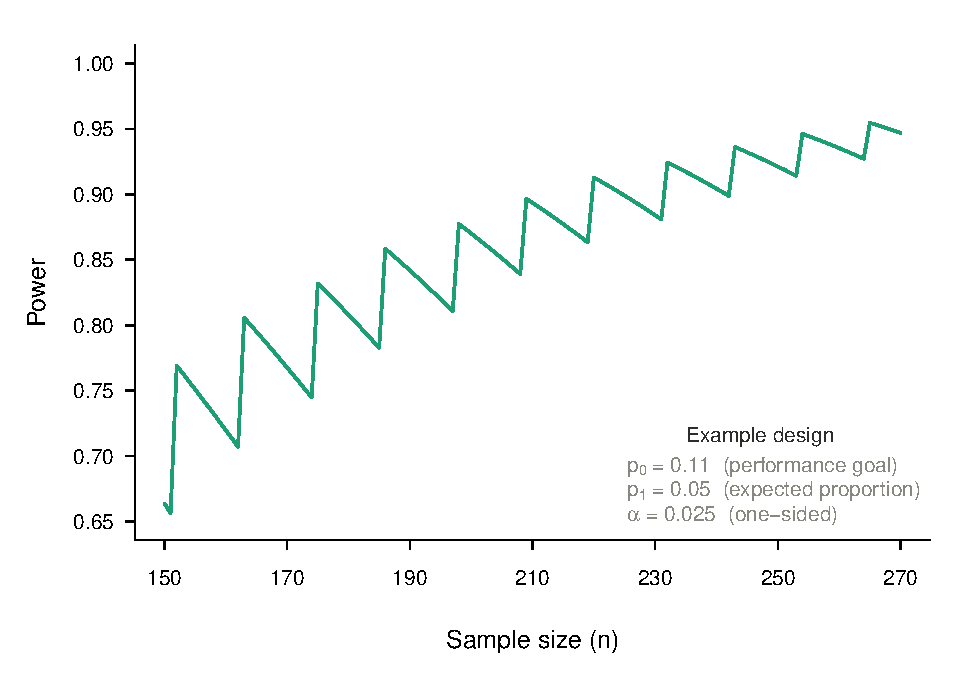
\includegraphics[width=0.8\linewidth]{Write_Up_Markdown_Script_files/figure-latex/sawtooth-power-1} 

}

\caption{Example saw-tooth power curve for a single-arm binary endpoint.}\label{fig:sawtooth-power}
\end{figure}

The required sample size can also be estimated through simulation. For
each candidate \(n\), a large number of trial datasets are generated
under the assumed true proportion \(p_1\), the selected confidence
interval method is applied to each, and power is estimated as the
proportion of simulated trials in which the decision rule is satisfied
(\citeproc{ref-international_council_for_harmonisation_statistical_1998}{5},\citeproc{ref-chow_sample_2017}{13}).
The required sample size is the smallest \(n\) at which this simulated
power meets the target
(\citeproc{ref-wang_leveraging_2021}{7},\citeproc{ref-chow_sample_2017}{13},\citeproc{ref-brown_interval_2001}{17}).
This approach is implemented in specialist software including PASS
(\citeproc{ref-noauthor_pass_nodate}{25}), nQuery
(\citeproc{ref-elashoff_nquery_nodate}{26}) and Cytel East
(\citeproc{ref-noauthor_east_nodate}{27}), as well as several R packages
(\citeproc{ref-noauthor_binomconfint_nodate}{28}), and is particularly
useful because it mirrors the planned analysis directly
(\citeproc{ref-wang_leveraging_2021}{7},\citeproc{ref-chow_sample_2017}{13}).

\subsection{Incorporating Prior Evidence: Bayesian Historical
Borrowing}\label{incorporating-prior-evidence-bayesian-historical-borrowing}

The frequentist sample size framework described in Section 4.2 treats
each trial as an isolated exercise, making no formal use of evidence
accumulated from comparable prior studies. Bayesian historical borrowing
offers an alternative by incorporating this prior evidence directly into
the analysis through a prior distribution, which is then updated with
current trial data to produce a posterior distribution
(\citeproc{ref-robert_harold_2009}{23},\citeproc{ref-campbell_bayesian_2011}{29},\citeproc{ref-ibrahim_power_2000}{30}).
In medical device studies, where single-arm designs are common and
exchangeable historical data from comparable devices may be available,
this approach can meaningfully reduce the required sample size
(\citeproc{ref-wang_single-arm_2024}{8},\citeproc{ref-cao_estimating_2025}{10},\citeproc{ref-campbell_bayesian_2011}{29}).

For a binary endpoint, a natural and tractable model uses the
Beta-Binomial conjugate structure
(\citeproc{ref-agresti_categorical_2013}{18},\citeproc{ref-robert_harold_2009}{23},\citeproc{ref-us_food_and_drug_administration_guidance_2010}{31}).
If historical data contribute \(\alpha_0\) observed events and
\(\beta_0\) observed non-events, the prior distribution is
(\citeproc{ref-ibrahim_power_2000}{30}):

\[p \sim \text{Beta}(\alpha_0, \beta_0)\]

After observing \(s\) events and \(f\) non-events in the current trial,
the posterior distribution is obtained by conjugate updating
(\citeproc{ref-robert_harold_2009}{23},\citeproc{ref-ibrahim_power_2000}{30},\citeproc{ref-us_food_and_drug_administration_guidance_2010}{31}):

\[p \mid s, f \sim \text{Beta}(\alpha_0 + s,\; \beta_0 + f)\]

This posterior combines historical and current evidence into a single
updated estimate of the true event probability. The influence of the
prior relative to the current data is often summarised by its Effective
Sample Size (ESS), which approximates the number of current observations
the prior is equivalent to
(\citeproc{ref-robert_harold_2009}{23},\citeproc{ref-ibrahim_power_2000}{30},\citeproc{ref-us_food_and_drug_administration_guidance_2010}{31}).
A prior with a large ESS concentrates the posterior more tightly around
the historical estimate, potentially reducing the number of current
patients needed to reach a given level of precision or power
(\citeproc{ref-us_food_and_drug_administration_guidance_2010}{31}).

The central assumption underlying any borrowing strategy is
exchangeability --- the requirement that the historical and current
populations are sufficiently similar that combining information across
them is scientifically justified
(\citeproc{ref-us_food_and_drug_administration_guidance_2010}{31},\citeproc{ref-chiaruttini_bayesian_2025}{32}).
Where full exchangeability cannot be assumed, partial borrowing
approaches allow the historical contribution to be downweighted
(\citeproc{ref-ibrahim_power_2000}{30},\citeproc{ref-chiaruttini_bayesian_2025}{32}).
The power prior of Ibrahim and Chen (2000) formalises this by raising
the historical likelihood to a discounting factor \(a_0 \in [0,1]\)
before forming the prior, with \(a_0 = 1\) representing full borrowing
and \(a_0 = 0\) representing no borrowing
(\citeproc{ref-ibrahim_power_2000}{30}). Adaptive borrowing methods take
a data-driven approach, adjusting the degree of borrowing based on the
observed compatibility between historical and current data ---
increasing borrowing when the two are consistent and reducing it when
they diverge
(\citeproc{ref-us_food_and_drug_administration_guidance_2010}{31},\citeproc{ref-chiaruttini_bayesian_2025}{32}).

Because borrowing can affect operating characteristics including Type I
error and power, its properties must be evaluated through simulation
across a range of plausible scenarios before the design is finalised
(\citeproc{ref-us_food_and_drug_administration_guidance_2010}{31}--\citeproc{ref-gamble_guidelines_2017}{33}).
Regulatory guidance on Bayesian statistics in medical device trials
recognises the potential for historical borrowing to reduce sample size
requirements while emphasising that the assumptions underlying the prior
must be clinically and statistically justified
(\citeproc{ref-campbell_bayesian_2011}{29},\citeproc{ref-us_food_and_drug_administration_guidance_2010}{31}).
Section 4.4 applies this framework to the BioMimics 3D safety endpoint
by incoperating the historical evidence derived in Section 5.1.

\subsection{Statistical Analysis Plans in Clinical
Trials}\label{statistical-analysis-plans-in-clinical-trials}

A Statistical Analysis Plan (SAP) is a formal document that provides a
detailed and technical description of the statistical methods to be used
in the analysis of a clinical trial, elaborating on the approaches
outlined in the study protocol
(\citeproc{ref-gamble_guidelines_2017}{33},\citeproc{ref-fradera_statistical_2024}{34}).
According to ICH E9, the SAP should be finalised before the unblinded
review of data, ensuring that all analytical decisions are made
independently of the observed results
(\citeproc{ref-international_council_for_harmonisation_statistical_1998}{5}).
This requirement exists because statistical analysis involves choices
about endpoints, methods, populations and decision rules that can
influence the study's conclusions. Pre-specifying those choices reduces
the risk of bias and of inflated Type I error while promoting
transparency, reproducibility and scientific integrity.

Pre-specification is a cornerstone of reproducible clinical research and
is expected by regulatory bodies, including the FDA and EMA, in
submissions supporting a marketing authorisation
(\citeproc{ref-international_council_for_harmonisation_statistical_1998}{5},\citeproc{ref-noauthor_medical_2026}{11},\citeproc{ref-kahan_how_2020}{35}).
In single-arm designs, where the absence of randomisation provides less
protection against bias, a rigorously developed SAP is particularly
important, and any deviations from it must be transparent and justified
(\citeproc{ref-schulz_sample_2005}{14},\citeproc{ref-gamble_guidelines_2017}{33}).
Without a concurrent control group, the conclusion relies on comparing
the observed outcomes against a pre-specified benchmark. Consequently,
key elements of this comparison --- namely the performance goal value,
confidence interval method and assumptions underlying the sample size
calucaltion --- can each independently alter the conclusion
(\citeproc{ref-wang_leveraging_2021}{7},\citeproc{ref-cao_estimating_2025}{10},\citeproc{ref-kahan_how_2020}{35}).

The implications of these methodological choices for sample size
requirements and study feasibility are examined thorugh the BioMimics 3D
case study presented throughout this thesis.

\section{Case Study and Data Sources}\label{case-study-and-data-sources}

\subsection{BioMimics 3D Vascular
Stent}\label{biomimics-3d-vascular-stent}

The BioMimics 3D vascular stent was selected as the primary case study
throughout this analysis. The device is a self-expanding, permanent
bare-metal nitinol stent developed for the treatment of femoropopliteal
Peripheral Artery Disease (PAD), a condition characterised by
atherosclerotic narrowing of the arteries supplying the lower limb
(\citeproc{ref-rammos_biomimics_2024}{36}--\citeproc{ref-zeller_helical_2016}{38}).
In this setting, successful treatment is defined by achieving initial
vessel patency and maintaining clinical benefit over time without
restenosis, reintervention, amputation or major adverse events
(\citeproc{ref-rocha-singh_performance_2007}{9},\citeproc{ref-rammos_biomimics_2024}{36},\citeproc{ref-tepe_local_2008}{39}).

Unlike conventional straight stents, the BioMimics 3D stent incorporates
a helical geometry intended to mimic the natural curvature and movement
of the femoropopliteal artery
(\citeproc{ref-rammos_biomimics_2024}{36},\citeproc{ref-zeller_helical_2016}{38}).
This design is hypothesised to promote blood flow patterns within the
treated vessel and reduce the risk of restenosis after implantation
(\citeproc{ref-rammos_biomimics_2024}{36},\citeproc{ref-zeller_helical_2016}{38}).
Consequently, clinically meaningful outcomes such as Target Vessel
Revascularisation (TVR), amputation and changes in Rutherford
classification are important measures of the device's ability to provide
sustained therapeutic benefit in patients with symptomatic PAD
(\citeproc{ref-rocha-singh_performance_2007}{9},\citeproc{ref-rammos_biomimics_2024}{36},\citeproc{ref-laird_nitinol_2010}{37}).

Initial meetings with the lead scientist involved in the BioMimics
development helped clarify the purpose of the device, the interpretation
of clinically meaningful performance, and the practical and statistical
constraints most relevant to the design of the pivotal study. This
demonstrates the importance of clinical knowledge in informing the
statistical design of the trial
(\citeproc{ref-schumi_through_2011}{1},\citeproc{ref-international_council_for_harmonisation_statistical_1998}{5},\citeproc{ref-wang_leveraging_2021}{7}).
It is clinicians and scientists who determine key design assumptions
such as the expected performance of BioMimics, sample size requirements,
anticipated dropout rates, and other practical considerations that
influence study design. Performance goals, endpoints and a sample size
that are mathematically convenient but lack clinical relevance do not
provide a robust basis for evaluating the device
(\citeproc{ref-international_council_for_harmonisation_statistical_1998}{5},\citeproc{ref-wang_leveraging_2021}{7},\citeproc{ref-rocha-singh_performance_2007}{9}).

\subsection{Endpoints}\label{endpoints}

Endpoint selection was guided by two criteria: clinical relevance to
femoropopliteal disease and sufficient historical literature to support
defensible performance goals
(\citeproc{ref-wang_leveraging_2021}{7},\citeproc{ref-rocha-singh_performance_2007}{9}).
Candidate endpoints were identified through a targeted review of
comparable peripheral vascular device trials and the 2007 guidance
document by Rocha-Singh et al.~on behalf of VIVA Physicians, which
synthesised evidence from three studies of femoropopliteal bare nitinol
stents and served as the primary regulatory reference point for this
analysis
(\citeproc{ref-rocha-singh_performance_2007}{9},\citeproc{ref-laird_nitinol_2010}{37},\citeproc{ref-zeller_helical_2016}{38}).

For safety, candidate endpoints were assessed at 30 days and included
all-cause mortality, major amputation and TVR. These were combined into
a single composite endpoint because each component represents a
clinically significant harm and individually the events occur too
infrequently to yield stable estimates
(\citeproc{ref-rocha-singh_performance_2007}{9},\citeproc{ref-rammos_biomimics_2024}{36},\citeproc{ref-laird_nitinol_2010}{37}).

For efficacy, candidate endpoints were assessed at 12 months. Rutherford
classification, a clinical scale describing the severity of PAD
symptoms, was selected because it captures patient-level disease status
rather than purely anatomical outcomes
(\citeproc{ref-rocha-singh_performance_2007}{9},\citeproc{ref-laird_nitinol_2010}{37}).
Specifically, improvement or no deterioration in Rutherford score from
post-intervention baseline was used, as this reflects whether patients
experienced meaningful clinical benefit over the follow-up period
(\citeproc{ref-rocha-singh_performance_2007}{9},\citeproc{ref-rammos_biomimics_2024}{36}).

The selected endpoints were therefore the 30-day composite of all-cause
mortality, major amputation and TVR for safety, and improvement or no
deterioration in Rutherford classification score at 12 months for
efficacy.

\subsection{Literature Search and Meta-analysis
Data}\label{literature-search-and-meta-analysis-data}

The same guidance document was used to determine justifiable performance
goal values for both the safety and efficacy endpoints.

For each relevant study, aggregate-level outcome data were extracted.
This included the number of patients experiencing the endpoint and the
number of patients assessed at the relevant follow-up time. Outcomes
were grouped according to endpoint definition and time point before
pooling. The time-point distinction was important because early safety
outcomes at 30 days and longer-term efficacy outcomes at 12 months
measure different aspects of device performance and cannot be combined
into a single estimate
(\citeproc{ref-rocha-singh_performance_2007}{9},\citeproc{ref-rammos_biomimics_2024}{36}).

A logit transformation was used to stabilise the variance before
pooling. This was required as the outcomes were binary proportions and
because the extreme event proportions expected create boundary settings
where raw proportions can behave poorly
(\citeproc{ref-wang_leveraging_2021}{7},\citeproc{ref-brown_interval_2001}{17}).

A generalised linear mixed model with a binomial likelihood was applied
to pool study-level proportions. This approach was selected because the
extracted data consisted of event counts versus study sample sizes and
handled extreme proportions more appropriately than simple normal
approximations. A random-effects structure was employed to allow for
between-study heterogeneity rather than assuming that all studies
estimated the same underlying event proportion. This was important
because the historical studies differed in design, population, endpoint
reporting and follow-up
(\citeproc{ref-wang_leveraging_2021}{7},\citeproc{ref-cao_estimating_2025}{10}).

The resulting estimates used to construct candidate performance goals
were as follows. For the 30-day safety composite endpoint, the pooled
estimate was approximately 6\%, with the upper confidence limit
extending to approximately 12\%. Values between the pooled point
estimate and the upper confidence limit were considered as the safety
performance goal, giving a benchmark of approximately 6--12\% for the
maximum acceptable proportion of patients with an early composite event.
For the 12-month stable or improved Rutherford classification endpoint,
the pooled estimate was approximately 95.8\%, with the lower confidence
limit extending to approximately 88\%. Values between the pooled point
estimate and the lower confidence limit were considered as the efficacy
performance goal, giving a benchmark of approximately 88--95.8\% for the
minimum acceptable proportion of patients with stable or improved
Rutherford classification.

\subsection{Derivation of Performance
Goals}\label{derivation-of-performance-goals}

In principle, the pooled point estimate from the historical studies
represents the weighted average or best estimate of expected performance
in the available evidence. However, using the point estimate directly as
the performance goal would ignore uncertainty in the historical data
(\citeproc{ref-wang_leveraging_2021}{7}). This is problematic when the
available evidence may be based on a small number of studies with
limited sample sizes and differing endpoint definitions
(\citeproc{ref-international_council_for_harmonisation_statistical_1998}{5},\citeproc{ref-wang_leveraging_2021}{7},\citeproc{ref-cao_estimating_2025}{10}).

For this reason, the proposed performance goals in this study were based
on confidence interval boundaries rather than the pooled point
estimates. For the safety endpoint, the upper confidence limit was
proposed because higher event proportions represent worse performance.
For the efficacy endpoint, the lower confidence limit was proposed
because lower event proportions represent worse performance. This
provided a conservative estimate incorporating the uncertainty in the
historical event proportions
(\citeproc{ref-wang_leveraging_2021}{7},\citeproc{ref-rocha-singh_performance_2007}{9}).

\newpage

\section{Methods}\label{methods}

\subsection{Simulation Study}\label{simulation-study}

To evaluate the confidence interval methods introduced in Section 2.3, a
simulation study was designed following the approach of Pires \& Amado
(2008) (\citeproc{ref-pires_interval_2008}{22}). The aim was to compare
coverage probability and expected interval width across a range of true
event proportions and sample sizes, before applying these methods within
the performance goal framework (\citeproc{ref-pires_interval_2008}{22}).

For each scenario, the number of observed events was assumed to follow a
binomial distribution,

\[X \sim \text{Binomial}(n, p)\]

where \(X\) is the number of observed events, \(n\) is the sample size
and \(p\) is the true underlying event probability
(\citeproc{ref-brown_interval_2001}{17}). Rather than evaluating
performance at a single fixed proportion, a grid of true proportions was
used to examine interval behaviour across a range of clinically
plausible event proportions. Given that the BioMimics 3D endpoints
involve either low complication or high success proportions, the
simulation focused on the range
(\citeproc{ref-brown_interval_2001}{17},\citeproc{ref-pires_interval_2008}{22}):

\[p \in \{0.001, 0.002, \ldots, 0.200\}\]

Methods were evaluated at three sample sizes, \(n = 20\), 50 and 100,
reflecting the small to moderate study sizes typical of single-arm
performance goal studies
(\citeproc{ref-wang_leveraging_2021}{7},\citeproc{ref-wang_single-arm_2024}{8}).

For each combination of \(n\), \(p\) and confidence interval method, the
confidence limits were calculated across all possible values of \(X\).
Two operating characteristics were then used to assess performance:
coverage probability and expected interval width
(\citeproc{ref-brown_interval_2001}{17},\citeproc{ref-pires_interval_2008}{22}).

Coverage probability is the probability that the constructed interval
contains the true value of \(p\)
(\citeproc{ref-brown_interval_2001}{17}):

\[\text{CP}(p) = P_p\!\left(L(X,n) \leq p \leq U(X,n)\right)\]

where \(L(X,n)\) and \(U(X,n)\) are the lower and upper confidence
limits. Since the target nominal level was 95\%, a well-performing
method should produce coverage close to 0.95 across the evaluated range.
To summarise behaviour across the full grid, both the average coverage
probability and the minimum coverage probability were recorded:

\[\overline{CP} = \frac{1}{m} \sum_{j=1}^{m} CP(p_j)\]

\[CP_{\min} = \min_{1 \leq j \leq m} CP(p_j)\]

The average captures typical performance, while the minimum identifies
whether any method fell substantially below the nominal level at
specific values of \(p\).

Expected interval width was used as a measure of precision. For a given
true proportion, sample size and method, the expected width was
calculated as:

\[E_p[W(X,n)] = \sum_{x=0}^{n} \{U(x,n) - L(x,n)\} \binom{n}{x} p^x (1-p)^{n-x}\]

and averaged across the simulation grid to give an overall summary of
interval length for each method
(\citeproc{ref-brown_interval_2001}{17},\citeproc{ref-pires_interval_2008}{22}):

\[\bar{W} = \frac{1}{m} \sum_{j=1}^{m} E_{p_j}[W(X,n)]\]

Results were summarised graphically. Coverage probability was plotted
against the true proportion \(p\) for each method and sample size, with
a dashed reference line at the nominal 95\% level. Combined plots were
also produced to allow direct comparison across methods on the same
axes. A second set of plots compared average coverage probability
against average expected interval width, providing a summary of the
trade-off between reliability and precision for each method. The
findings from this simulation informed the selection of confidence
interval methods used in the sample size calculations in Section 4.2.

\subsection{Sample Size Calculation}\label{sample-size-calculation}

Sample size calculations were carried out for the BioMimics 3D case
study using the single-arm performance goal framework described in
Section 2.4
(\citeproc{ref-wang_leveraging_2021}{7},\citeproc{ref-rocha-singh_performance_2007}{9}).
The endpoints, performance goal values, and assumed true event
proportion were informed by the meta-analysis and clinical discussions
described in Sections 3.1 and 3.3, with results reported in Section 5.3.

A target power of 90\% was used throughout, which is conventional in
medical device studies where 80\% power, common in pharmaceutical
trials, is considered insufficient to support a regulatory submission
(\citeproc{ref-chow_sample_2017}{13},\citeproc{ref-wang_sample_2020}{16},\citeproc{ref-julious_sample_2004}{24},\citeproc{ref-us_food_and_drug_administration_guidance_2010}{31}).
A one-sided significance level of \(\alpha = 0.025\) corresponding to a
one sided 97.5\% confidence interval and consistent with the decision
rule described in Section 2.2 was
used(\citeproc{ref-oczkowski_clinicians_2014}{3},\citeproc{ref-us_food_and_drug_administration_guidance_2010}{31}).

Sample size was determined through simulation rather than closed-form
calculation, as exact analytical solutions are not always available when
the confidence interval method forms part of the decision rule
(\citeproc{ref-chow_sample_2017}{13},\citeproc{ref-brown_interval_2001}{17},\citeproc{ref-agresti_approximate_1998}{19}).
Simulation provides a flexible alternative that mirrors the planned
primary analysis directly and is the approach implemented in PG-Power,
described in Section 4.3.

\subsection{Shiny Application:
PG-Power}\label{shiny-application-pg-power}

PG-Power is an interactive R Shiny application developed as part of this
thesis to implement the simulation-based sample size framework described
in Section 4.2 for single-arm performance goal studies. For each
candidate sample size, the application simulates a large number of
trials under the assumed true event proportion, applies the selected
confidence interval method, and estimates power as the proportion of
simulated trials satisfying the performance goal rule. The smallest
\(n\) achieving the target power is returned as the required sample
size.

The shiny app provided a transparent and reproducible implementation of
the sample size frame work, allowing the BioMimics 3D design assumptions
to be evaluated consistently across all six confidence interval methods.
By enabling users to simulate alternative study scenarios and visualise
the relationship between design assumptions, confidence interval choice,
required sample size and achieved power, PG-Power makes the sensitivity
of the design immediately visible. The integrated reporting function
further supports the pre specified decision-making shown to be necessary
in Aims 2 and 3. It allows study assumptions, outputs, visualisations
and interpretations to be documentedin a standardised report format. The
full report generated for the BioMimics 3D analysis is available in the
GitHub repository (see Appendix).

\subsection{Applying Bayesian Borrowing to the Safety
Endpoint}\label{applying-bayesian-borrowing-to-the-safety-endpoint}

The frequentist sample size calculations in Section 4.2 made no use of
the historical studies identified in Section 3.3 beyond their role in
deriving the performance goal. This section examines whether formally
incorporating that evidence as a prior distribution reduces the required
sample size relative to the frequentist result obtained in Section 5.3
(\citeproc{ref-campbell_bayesian_2011}{29},\citeproc{ref-us_food_and_drug_administration_guidance_2010}{31}).

To construct a concrete and interpretable prior, a hypothetical Phase II
dataset of 50 participants with 2 observed events was used, producing a
\(\text{Beta}(2, 48)\) prior with an estimated event proportion of
approximately 4\% and an ESS of 50
(\citeproc{ref-us_food_and_drug_administration_guidance_2010}{31}). The
choice of a hypothetical dataset rather than the historical studies
directly was deliberate. As the meta-analysis comprised of only three
studies of limited sample sizes, a fully justified prior would be
difficult to construct
(\citeproc{ref-ibrahim_power_2000}{30},\citeproc{ref-chiaruttini_bayesian_2025}{32},\citeproc{ref-gamble_guidelines_2017}{33}).
The hypothetical prior therefore serves as an illustrative example of
how borrowing would operate under plausible assumptions, rather than as
a formal design recommendation
(\citeproc{ref-campbell_bayesian_2011}{29},\citeproc{ref-chiaruttini_bayesian_2025}{32}).

Under the Beta-Binomial model introduced in Section 2.5, incorporating
\(s\) events and \(f\) non-events from the current trial updates the
prior to
(\citeproc{ref-robert_harold_2009}{23},\citeproc{ref-us_food_and_drug_administration_guidance_2010}{31}):

\[p \mid s, f \sim \text{Beta}(2 + s,\; 48 + f)\]

For inference, the posterior probability that the true event proportion
falls below the performance goal was evaluated against a decision
threshold of 0.95
(\citeproc{ref-campbell_bayesian_2011}{29},\citeproc{ref-us_food_and_drug_administration_guidance_2010}{31}):

\[P(p < p_0 \mid s, f) \geq 0.95\]

The required sample size was determined as the smallest \(n\) for which
this criterion was satisfied with at least 90\% probability under the
assumed true event proportion of 5\%, consistent with the frequentist
design assumptions in Section 4.2
(\citeproc{ref-chow_sample_2017}{13},\citeproc{ref-us_food_and_drug_administration_guidance_2010}{31}).

To examine sensitivity to prior weight, three prior distributions were
compared: \(\text{Beta}(0.2, 4.8)\), \(\text{Beta}(2, 48)\) and
\(\text{Beta}(20, 480)\), encoding the same event ratio of approximately
1:24 but corresponding to ESS of approximately 5, 50 and 500,
representing weak, moderate and strong borrowing respectively
(\citeproc{ref-ibrahim_power_2000}{30},\citeproc{ref-chiaruttini_bayesian_2025}{32},\citeproc{ref-gamble_guidelines_2017}{33}).

\newpage

\section{Results}\label{results}

\subsection{Meta-Analysis Results}\label{meta-analysis-results}

The meta-analysis of the three femoropopliteal bare nitinol stent
studies described in Section 3.3 produced pooled estimates for both
endpoints. The results are summarised in Figures 3 and 4.

\begin{table}[H]
\centering
\caption{\label{tab:performance-goals-table}Performance Goals for Safety and Efficacy}
\centering
\fontsize{11}{13}\selectfont
\begin{tabular}[t]{>{\raggedright\arraybackslash}p{5.2cm}cccc}
\toprule
\cellcolor[HTML]{3A3A6A}{\textcolor{white}{Endpoint}} & \cellcolor[HTML]{3A3A6A}{\textcolor{white}{Timepoint}} & \cellcolor[HTML]{3A3A6A}{\textcolor{white}{Pooled Proportion}} & \cellcolor[HTML]{3A3A6A}{\textcolor{white}{95\% CI}} & \cellcolor[HTML]{3A3A6A}{\textcolor{white}{Performance Goal}}\\
\midrule
\addlinespace[0.3em]
\multicolumn{5}{l}{\cellcolor[HTML]{4A4A6A}{\textcolor{white}{Safety Endpoints}}}\\
\hspace{1em}Composite (Death, Amputation, TVR) & 30 Days & 6.0\% & {}[2.9, 12.1\%] & $\leq$ 12\%\\
\addlinespace[0.3em]
\multicolumn{5}{l}{\cellcolor[HTML]{6B4A2A}{\textcolor{white}{Efficacy Endpoints}}}\\
\hspace{1em}RCC (Improved, No Change) & 12 Months & 95.8\% & {}[87.9, 98.6\%] & $\geq$ 88\%\\
\bottomrule
\end{tabular}
\end{table}

\begin{figure}[H]

{\centering 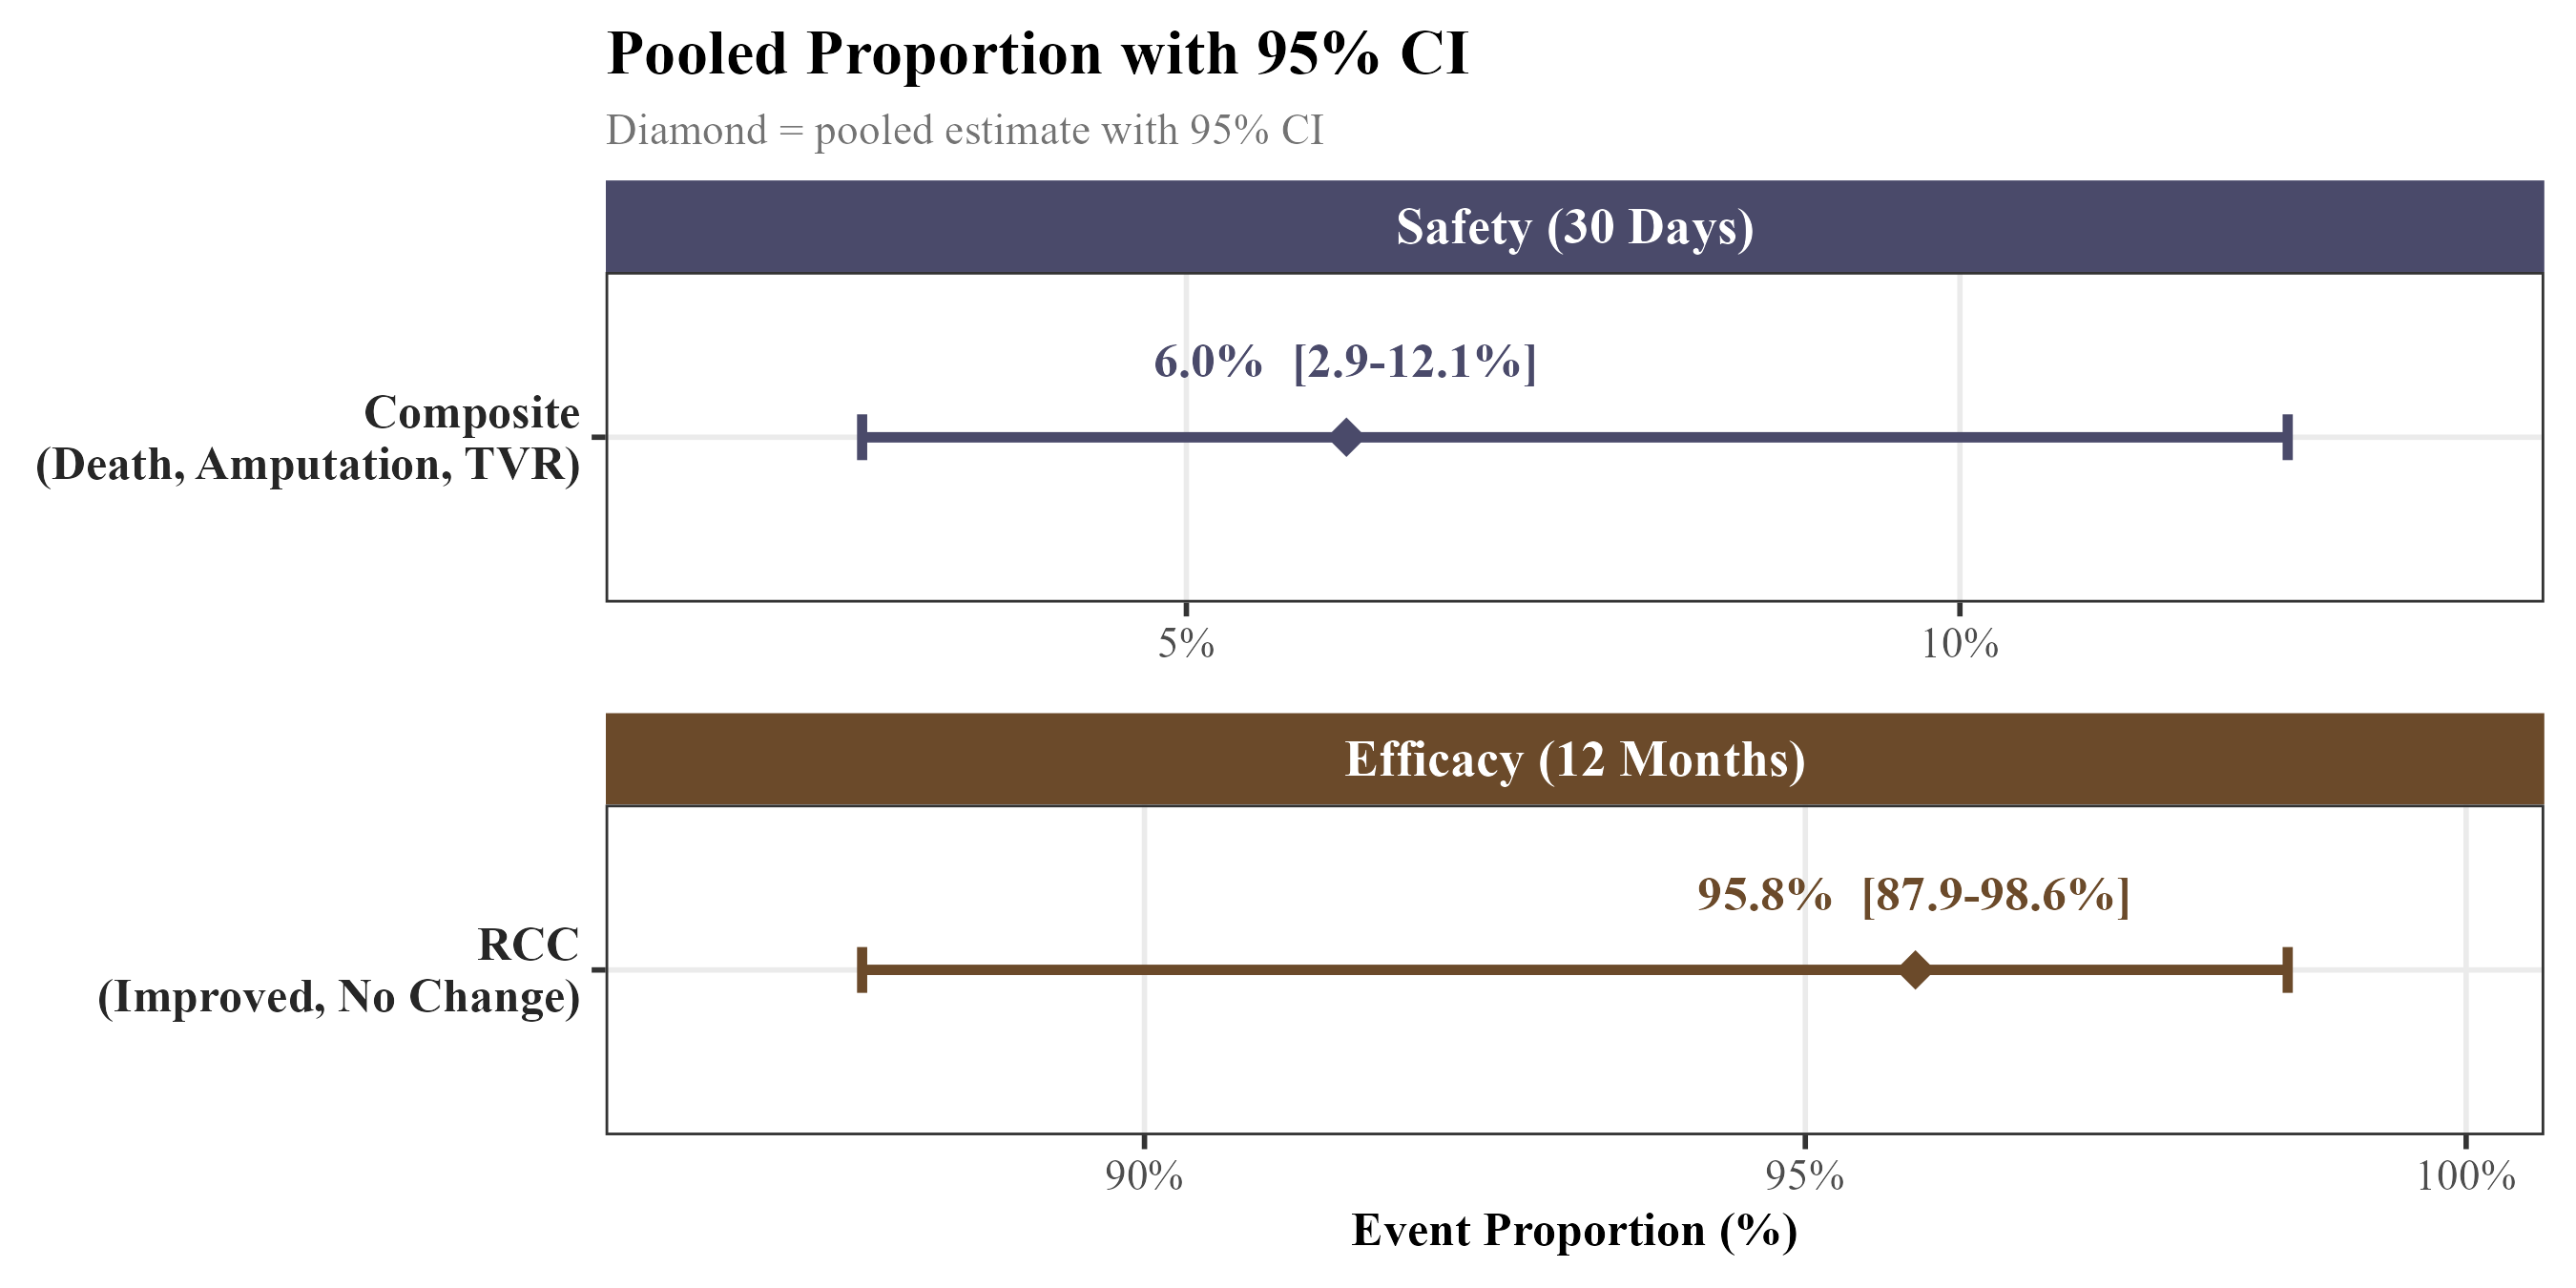
\includegraphics[width=0.8\linewidth]{Figures/forest_plot_pooled_estimates} 

}

\caption{Pooled event proportions with 95\% confidence intervals for the safety and efficacy endpoints.}\label{fig:forest-plot}
\end{figure}

The heterogeneity statistics for both endpoints are reported in Tables 2
and 3.

\begin{table}[H]
\centering
\caption{\label{tab:heterogeneity-A}Heterogeneity Statistics: 30-day Composite}
\centering
\fontsize{11}{13}\selectfont
\begin{tabular}[t]{>{\raggedright\arraybackslash}p{3cm}cc}
\toprule
\cellcolor[HTML]{3A3A6A}{\textcolor{white}{\textbf{Measure}}} & \cellcolor[HTML]{3A3A6A}{\textcolor{white}{\textbf{Value}}} & \cellcolor[HTML]{3A3A6A}{\textcolor{white}{\textbf{CI or p-value}}}\\
\midrule
$\tau^2$ & 0.00 & NA\\
$I^2$ & 0.0\% & 0.0\% to 0.9\%\\
H & 1.00 & 1.00 to 3.10\\
Q (Wald) & 0.00 & $p$ = 0.998\\
Q (LRT) & NA & NA\\
\bottomrule
\end{tabular}
\end{table}

\begin{table}[H]
\centering
\caption{\label{tab:heterogeneity-B}Heterogeneity Statistics: 12-month Rutherford classification}
\centering
\fontsize{11}{13}\selectfont
\begin{tabular}[t]{>{\raggedright\arraybackslash}p{3cm}cc}
\toprule
\cellcolor[HTML]{3A3A6A}{\textcolor{white}{\textbf{Measure}}} & \cellcolor[HTML]{3A3A6A}{\textcolor{white}{\textbf{Value}}} & \cellcolor[HTML]{3A3A6A}{\textcolor{white}{\textbf{CI or p-value}}}\\
\midrule
$\tau^2$ & 0.00 & NA\\
$I^2$ & 0.0\% & 0.0\% to 0.9\%\\
H & 1.00 & 1.00 to 3.10\\
Q (Wald) & 1.31 & $p$ = 0.520\\
Q (LRT) & NA & NA\\
\bottomrule
\end{tabular}
\end{table}

For both endpoints, the estimated between-study variance \(\tau^2\) was
0 and the \(I^2\) statistic was 0.0\% (95\% CI: 0.0--0.9\%), with
\(H = 1.00\). Cochran's Q test produced \(p\)-values of 0.998 and 0.520
for the safety and efficacy endpoints respectively. The implications of
these heterogeneity estimates for the interpretation of the derived
performance goals are discussed in Section 6.1.

\subsection{Simulation Study: CI Method
Comparison}\label{simulation-study-results}

Coverage probability was evaluated across a grid of true proportions
\(p \in \{0.001, \ldots, 0.200\}\) for each of the six confidence
interval methods at sample sizes \(n = 50\) and \(n = 100\). Results are
summarised through coverage probability curves and coverage-width
scatter plots.

\begin{figure}[H]

{\centering 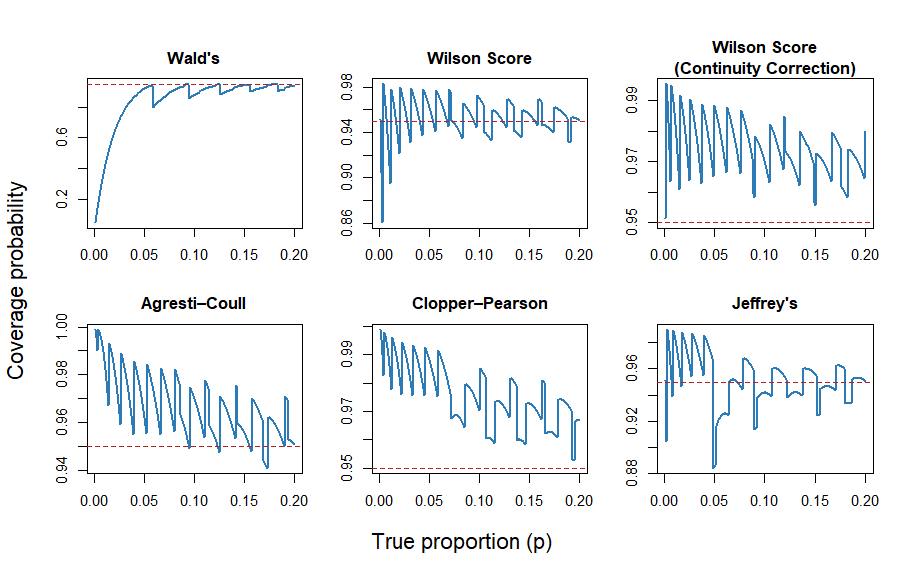
\includegraphics[width=1\linewidth]{Figures/coverage_probability_n50} 

}

\caption{Coverage probability curves for six binomial confidence interval methods at n = 50, evaluated across true proportions p in {0.001, ..., 0.200}. The dashed red line indicates the nominal 95\% level.}\label{fig:coverage-prob-n50}
\end{figure}

At \(n = 50\), the Wald interval produced coverage below 0.80 for true
proportions near zero, only approaching the nominal level near
\(p = 0.20\). The Wilson Score interval oscillated around 0.95, with
dips below 0.90 at low proportions near \(p = 0.001\) to 0.01. The
Jeffreys interval followed a similar pattern but with more pronounced
dips below nominal at low proportions. The Wilson Score with continuity
correction and Agresti-Coull interval maintained coverage above the
nominal level across virtually the entire proportion range. The
Clopper-Pearson interval was the most conservative, with coverage
remaining above 0.97 across nearly the entire evaluated range.

\begin{figure}[H]

{\centering 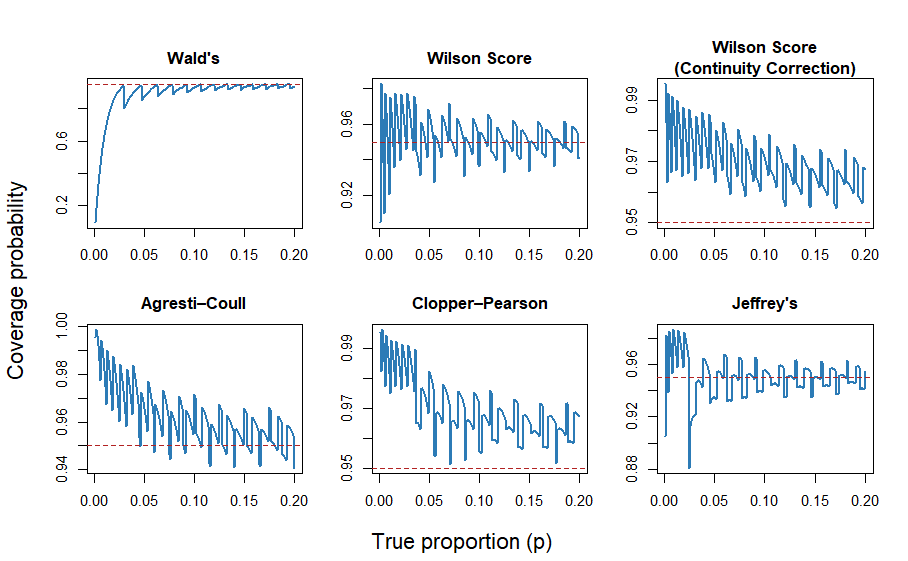
\includegraphics[width=1\linewidth]{Figures/coverage_probability_n100} 

}

\caption{Coverage probability curves for six binomial confidence interval methods at n = 100, evaluated across true proportions p in {0.001, ..., 0.200}. The dashed red line indicates the nominal 95\% level.}\label{fig:coverage-prob-n100}
\end{figure}

At \(n = 100\) the pattern was broadly similar. The Wald interval
remained well below 0.95 across most of the proportion range. The
remaining five methods continued to oscillate above the nominal level,
with Wilson Score and Jeffreys tracking closest to 0.95 and
Clopper-Pearson, Agresti-Coull and Wilson Score with continuity
correction remaining the most conservative.

\begin{figure}[H]

{\centering 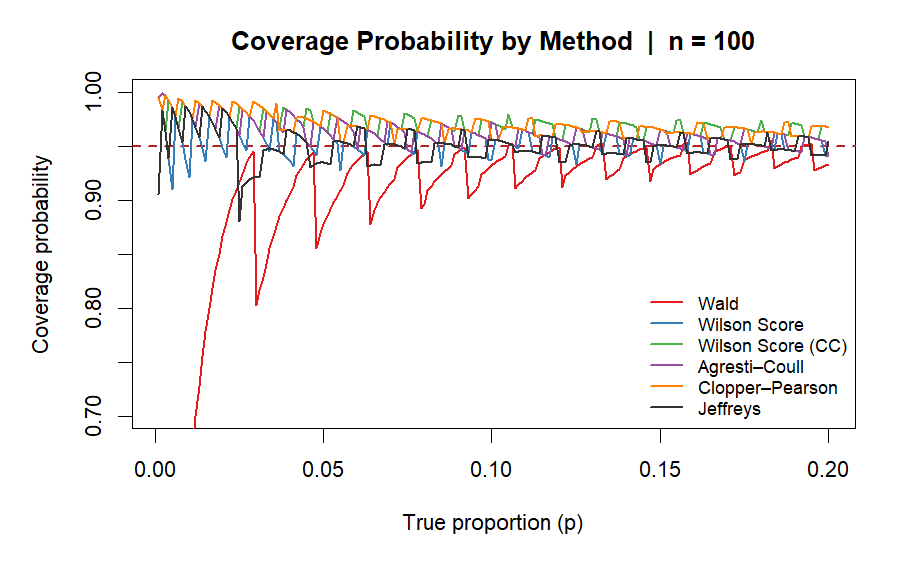
\includegraphics[width=1\linewidth]{Figures/coverage_probability_n100_overlay} 

}

\caption{Coverage probability curves for all six methods overlaid at n = 100. The dashed red line indicates the nominal 95\% level.}\label{fig:coverage-prob-overlay}
\end{figure}

The combined overlay for \(n = 100\) shows all six methods on the same
axes, illustrating the clear separation between the Wald interval and
the remaining five methods across the full proportion range.

The coverage-width scatter plots summarise the trade-off between average
coverage probability and average expected interval width at each sample
size.

\begin{figure}[H]

{\centering 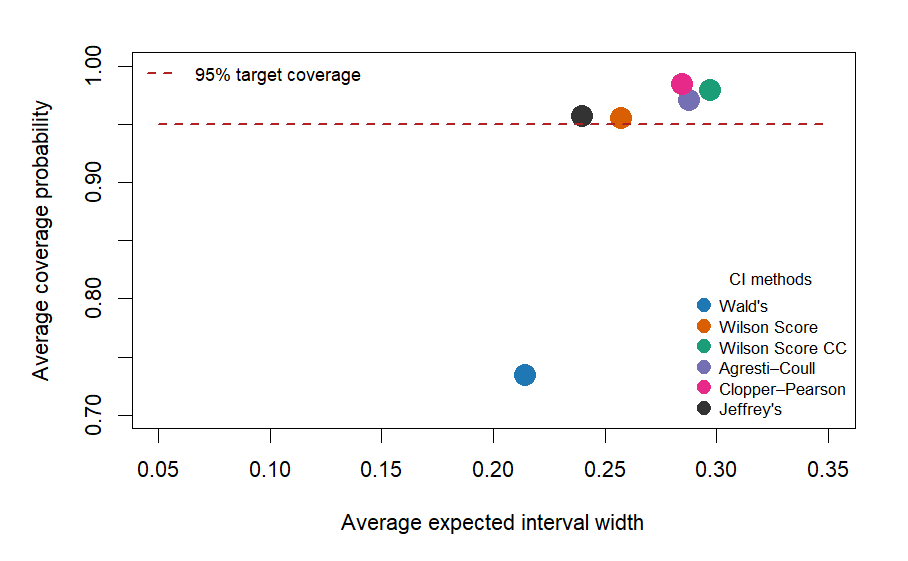
\includegraphics[width=0.8\linewidth]{Figures/coverage_width_n20} 

}

\caption{Average coverage probability against average expected interval width at n = 20.}\label{fig:coverage-width-n20}
\end{figure}

At \(n = 20\), the Wald interval produced average coverage of
approximately 0.73 with an average width of approximately 0.21. Wilson
Score and Jeffreys sat at or just above the nominal line with average
widths of approximately 0.24 and 0.25 respectively. Clopper-Pearson,
Agresti-Coull and Wilson Score with continuity correction sat above the
nominal line with average widths of approximately 0.29 and 0.30.

\begin{figure}[H]

{\centering 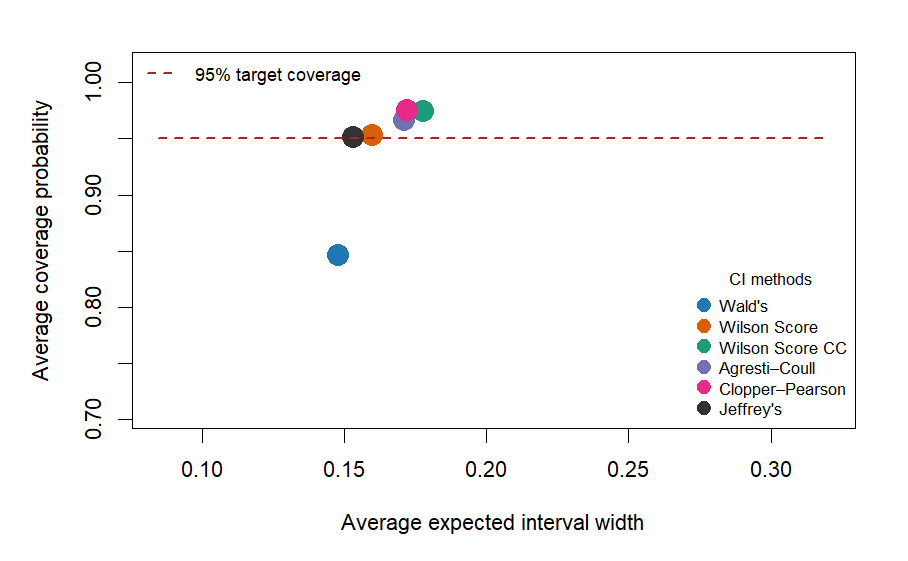
\includegraphics[width=0.8\linewidth]{Figures/coverage_width_n50} 

}

\caption{Average coverage probability against average expected interval width at n = 50.}\label{fig:coverage-width-n50}
\end{figure}

\begin{figure}[H]

{\centering 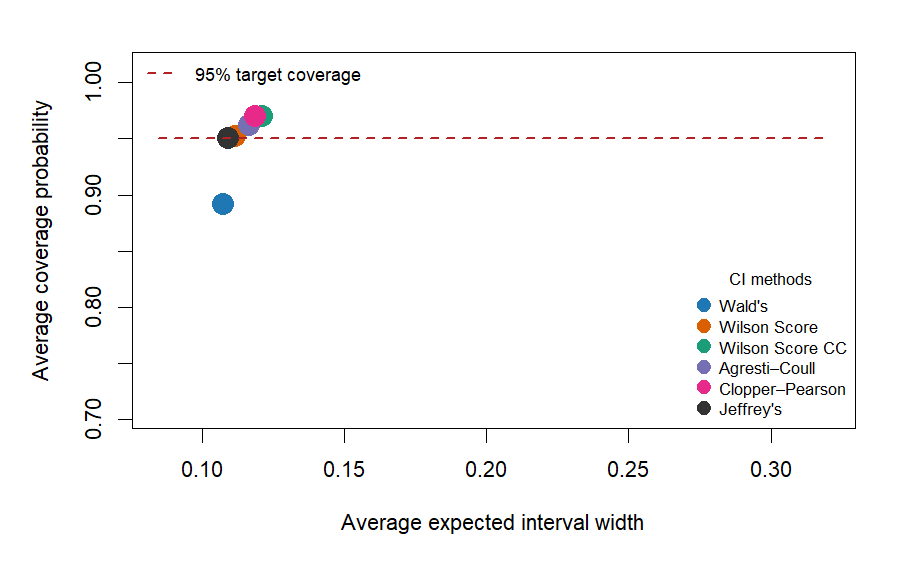
\includegraphics[width=0.8\linewidth]{Figures/coverage_width_n100} 

}

\caption{Average coverage probability against average expected interval width at n = 100.}\label{fig:coverage-width-n100}
\end{figure}

At \(n = 50\) and \(n = 100\) the five non-Wald methods converged, with
all five clustered near and above the nominal line in the coverage-width
plots. The ordering remained consistent across both sample sizes: Wilson
Score and Jeffreys sat closest to 0.95 with average widths of
approximately 0.16 and 0.11 at \(n = 50\) and \(n = 100\) respectively,
while Clopper-Pearson produced the widest average intervals at both
sample sizes.

\subsection{Sample Size and Confidence Interval Method
Comparison}\label{sample-size-and-confidence-interval-method-comparison}

Under the design assumptions established in Section 4.2, the required
sample size was determined using the single-arm performance goal
framework with an approved performance goal of \(p_0 = 0.11\), an
assumed true complication proportion of \(p_1 = 0.05\), a one-sided
significance level of \(\alpha = 0.025\) and a target power of 90\%. The
formal hypotheses were:

\[H_0: p \geq 0.11 \qquad H_1: p < 0.11\]

The Clopper-Pearson interval was used as the primary method for the main
sample size calculation. This choice was made partly on the basis of the
simulation results in Section 5.2, which showed Clopper-Pearson to be
the most conservative method with guaranteed nominal coverage, and
additionally because the exact binomial method underlying the
Clopper-Pearson interval is the default approach used in widely adopted
sample size software including PASS and nQuery
(\citeproc{ref-brown_interval_2001}{17},\citeproc{ref-clopper_use_1934}{20},\citeproc{ref-noauthor_pass_nodate}{25},\citeproc{ref-elashoff_nquery_nodate}{26}).

\begin{figure}[H]

{\centering 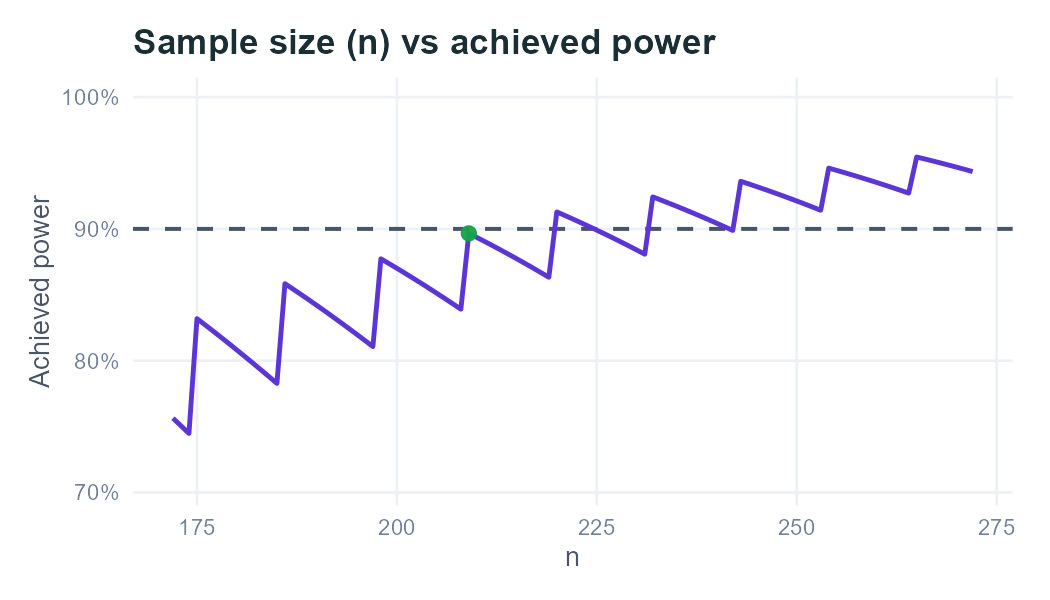
\includegraphics[width=0.9\linewidth]{Figures/power_curve_clopper_pearson} 

}

\caption{Power curve for the BioMimics 3D 30-day composite safety endpoint produced by PG-Power using the Clopper-Pearson method. The green point marks the required evaluable sample size of n = 209, at which achieved power was 89.7\%.}\label{fig:power-curve-cp}
\end{figure}

The required sample size varied across the six confidence interval
methods evaluated under the same design assumptions, as summarised in
the table below.

\begin{figure}[H]

{\centering 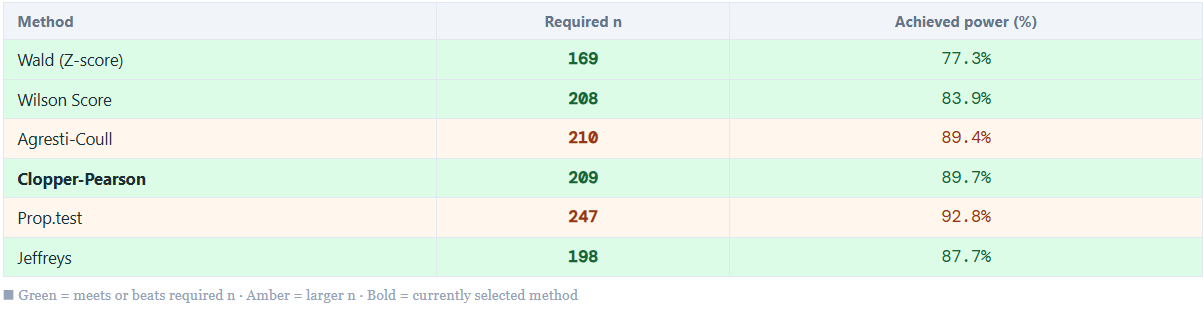
\includegraphics[width=0.8\linewidth]{Figures/sample_size_comparison_table} 

}

\caption{Required evaluable sample size and achieved power for six confidence interval methods under the BioMimics 3D safety endpoint design assumptions. Produced by PG-Power. Clopper-Pearson was set as the primary method.}\label{fig:sample-size-table}
\end{figure}

The Wald interval produced the smallest required sample size of 169
patients but achieved 77.3\% power under the assumed true complication
proportion, falling to meet the 90\% target. This is consistent with the
simulation results in Section 5.2, which showed systematic undercoverage
of the Wald interval across the relevant range of event proportions
(\citeproc{ref-brown_interval_2001}{17},\citeproc{ref-agresti_approximate_1998}{19}).
A sample size derived from the Wald interval would be unreliable as a
basis for study design.

Among the remaining methods, Jeffreys required 198 patients with
achieved power of 87.7\%, and Wilson Score required 208 patients at
83.9\% power, both falling below the 90\% target despite requiring
larger sample sizes. Clopper-Pearson and Agresti-Coull methods
approached the target power, requiring 209 and 210 patients with
achieved powers of 89.7\% and 89.4\% respectively. The Wilson Score with
continuity correction required the largest sample size of 247 patients,
achieving 92.8\% power, consistent with its conservative coverage
behaviour observed in Section 5.2.

Notably, Wilson Score required only one fewer patient than
Clopper-Pearson but achieved considerably lower power at 83.9\% versus
89.7\%. The difference between the Clopper-Pearson (209 patients) and
Wilson Score with continuity correction (247 patients), represents 38
additional evaluable patients or approximately 42 additional enrolments
after dropout adjustment.

\begin{figure}[H]

{\centering 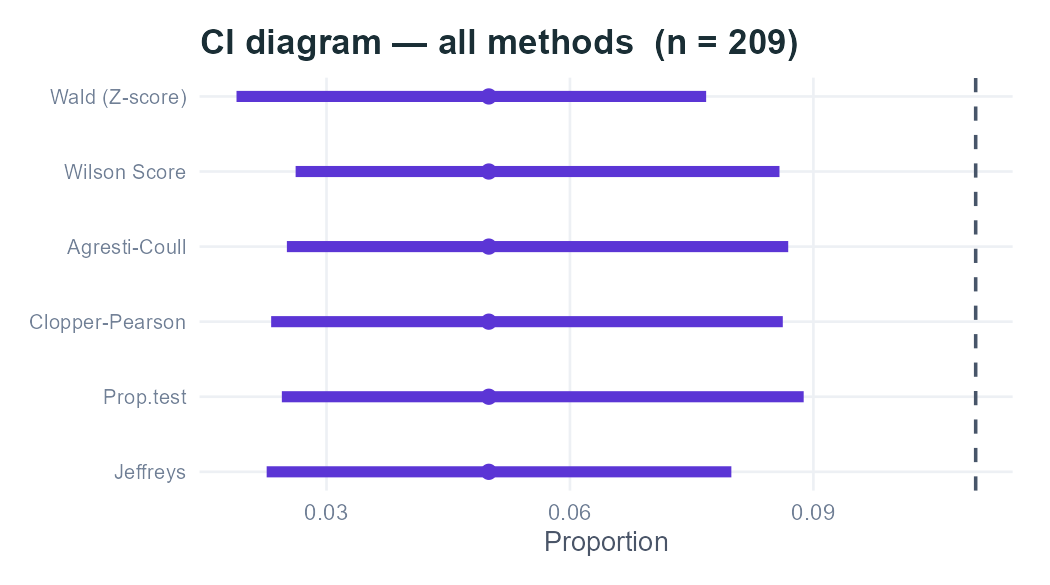
\includegraphics[width=1\linewidth]{Figures/ci_diagram_all_methods} 

}

\caption{Confidence intervals for the observed event proportion across all six methods at n = 209. Produced by PG-Power under the BioMimics 3D safety endpoint design assumptions. The dashed vertical line indicates the performance goal of 11\%.}\label{fig:ci-diagram}
\end{figure}

A full report generated by the PG-Power application for these design
assumptions, including power curves and sensitivity analyses, is
available in PDF form on the project GitHub repository (see Appendix).

\subsection{Bayesian Historical Borrowing
Results}\label{bayesian-historical-borrowing-results}

Under the \(\text{Beta}(2, 48)\) prior and the design assumptions
described in Section 4.4, the required evaluable sample size was
\(n = 79\), permitting no more than 4 observed events. This represents a
reduction of 130 patients, approximately 62\%, relative to the
Clopper-Pearson frequentist result of 209 from Section 5.3.

\begin{figure}[H]

{\centering 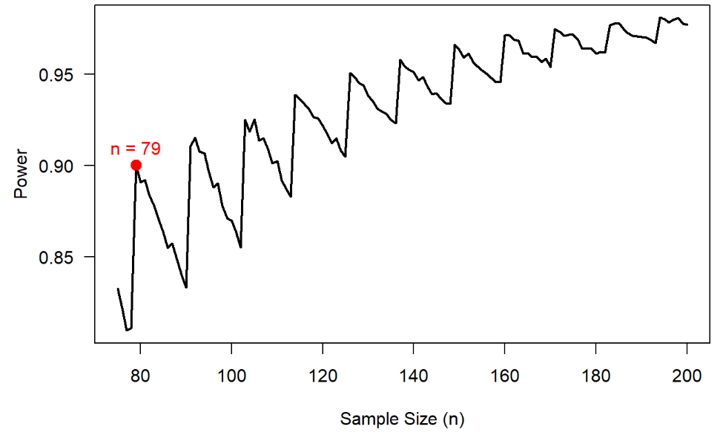
\includegraphics[width=0.9\linewidth]{Figures/bayesian_power_curve} 

}

\caption{Bayesian power curve for the BioMimics 3D 30-day composite safety endpoint under a Beta(2, 48) prior (performance goal p0 = 0.11, assumed true proportion p1 = 0.05, one-sided alpha = 0.025, decision threshold 0.95, target power 90\%).}\label{fig:bayesian-power}
\end{figure}

The power curve illustrates how achieved power evolves across candidate
sample sizes under the Bayesian model. The saw-tooth pattern reflects
the same discrete stepwise behaviour described in Section 2.4, where
power decreases gradually within ranges of \(n\) and increases sharply
when an additional event becomes permissible. The required sample size
of 79 corresponds to the first point at which the power curve crosses
the 90\% threshold.

The sensitivity of this result to prior weight is shown in the figure
below. All three distributions, \(\text{Beta}(0.2, 4.8)\),
\(\text{Beta}(2, 48)\) and \(\text{Beta}(20, 480)\), encode the same
underlying event ratio but differ substantially in how strongly they
concentrate the posterior.

\begin{figure}[H]

{\centering 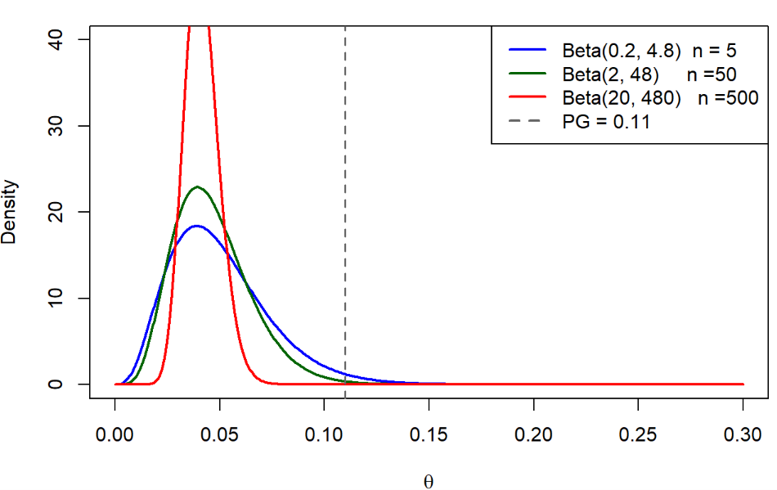
\includegraphics[width=0.9\linewidth]{Figures/prior_weight_sensitivity} 

}

\caption{Effect of prior weight on the posterior distribution of the true event proportion theta under three Beta priors with the same event ratio (1:24).}\label{fig:prior-weight}
\end{figure}

With ESS = 5 the posterior is broad and driven largely by the current
data, offering modest sample size reduction relative to the frequentist
result. With ESS = 50 the posterior concentrates more clearly around the
historical event proportion of 4\%, well below the performance goal of
11\%, producing the reduction to \(n = 79\) reported above. With ESS =
500 the posterior is narrow and the prior dominates, largely overriding
the current trial data. While this produces the greatest reduction in
required sample size, it also renders the conclusion highly sensitive to
the validity of the historical data and the exchangeability assumption.
If the true event proportion in the current study differs from the
historical estimate, a strongly informative prior will pull the
posterior toward the historical value regardless of what the current
data show. Similarly, the substantial reductions in required sample size
correspond to the favourable historical event proportion of 0.04. If the
historical event proportion were less favourable or closer to the
pre-specified threshold, the resulting reduction in required sample size
would be more modest.

\newpage

\section{Discussion}\label{discussion}

\subsection{Interpretation of Main
Findings}\label{interpretation-of-main-findings}

This study set out to examine how performance goal selection, confidence
interval choice and the assumptions underlying the sample size
calculation interact to influence design requirements and conclusions in
a single-arm performance goal medical device setting. The five aims
established in Section 1.5 are addressed in turn before their combined
implications are considered.

\subsubsection{Aim 1: Deriving Evidence-Based Performance Goals Through
Meta-Analysis}\label{aim-1-deriving-evidence-based-performance-goals-through-meta-analysis}

The meta-analysis of three historical femoropopliteal nitinol stent
studies yielded a pooled 30-day composite complication proportion of
approximately 6\%, with the upper confidence limit extending to 12\%,
and a pooled 12-month Rutherford classification success proportion of
approximately 95.8\%, with the lower confidence limit at 88\%.
Confidence interval boundaries rather than point estimates were used to
derive the proposed performance goals, acknowledging the uncertainty
inherent in a small historical evidence base of only three studies and
116 patients combined. The resulting benchmark values of 12\% for safety
and 88\% for efficacy are therefore point selections derived from ranges
of plausible values, with the width of these ranges reflecting the
limited precision of the available evidence.

Although using confidence interval limits protects against incorrectly
concluding that an effective device does not meet the performance
requirement, the choice of benchmark has important consequences for
study design and interpretation. First, the value of the selected
performance goal within the plausible range of values matters: the
sensitivity of sample size requirements to the difference between the
proposed 12\% and approved 11\% thresholds is examined in Aim 3. Second,
deriving performance goals from conservative confidence interval
boundaries rather than point estimates can introduce biocreep
(\citeproc{ref-eversonstewart_biocreep_2010}{40}). If successive device
generations are each evaluated against benchmarks derived from
increasingly conservative historical estimates, acceptable performance
standards may gradually drift from the original level of clinical
effectiveness. This risk is amplified in a single-arm study because
there is no active comparator to anchor the comparison
(\citeproc{ref-wang_leveraging_2021}{7},\citeproc{ref-cao_estimating_2025}{10}).
Therefore the validity of the derived benchmarks ultimately depends on
the statistical evidence with clinical and regulatory judgement, as
methodological approaches alone cannot substitute for clinical context.

\subsubsection{Aim 2: Comparing Confidence Interval Methods for Binary
Endpoints}\label{aim-2-comparing-confidence-interval-methods-for-binary-endpoints}

The simulation study confirmed that confidence interval method choice
has a meaningful and consistent effect on coverage behaviour at the low
event proportions, relevant to the BioMimics 3D safety endpoint. The
Wald interval consistently fell below the nominal 95\% level, with
average coverage of approximately 0.73 at \(n = 20\), 0.84 at \(n = 50\)
and 0.89 at \(n = 100\). This undercoverage was not accompanied by any
compensating gain in precision: the Wald interval produced average
widths comparable to better-performing methods while failing to meet the
nominal level throughout. Although its poor behaviour at extreme
proportions is well documented in the literature, its inclusion here
serves a practical purpose by demonstrating that a method commonly
applied by default in standard software would produce unreliable results
in this setting
(\citeproc{ref-brown_interval_2001}{17},\citeproc{ref-agresti_approximate_1998}{19}).

Among the remaining five methods, Wilson Score and Jeffreys sat closest
to the nominal level with the narrowest intervals, while
Clopper-Pearson, Agresti-Coull and the continuity-corrected Wilson Score
were consistently conservative with progressively wider intervals. Both
Wilson Score and Jeffreys showed dips below the nominal level at very
low proportions near \(p = 0.001\) to 0.01
(\citeproc{ref-brown_interval_2001}{17},\citeproc{ref-pires_interval_2008}{22}),
which is directly relevant given the expected complication proportion
for the BioMimics 3D safety endpoint. The ordering of methods was stable
across all sample sizes, providing a consistent basis for method
selection in the calculations that followed.

\subsubsection{Aim 3: Evaluating the Effect of Performance Goal and
Interval Choice on Sample
Size}\label{aim-3-evaluating-the-effect-of-performance-goal-and-interval-choice-on-sample-size}

The sample size results demonstrated that neither the performance goal
nor the confidence interval method can be treated as a neutral design
choice. Under the approved performance goal of 11\% and an assumed true
complication proportion of 5\%, the required evaluable sample size
ranged from 169 patients under the Wald interval, which failed to meet
the 90\% power target, to 247 under the continuity-corrected Wilson
Score. Among the methods approaching the power target, Clopper-Pearson
required 209 patients at 89.7\% power and Agresti-Coull required 210 at
89.4\%, while Jeffreys required 198 patients at 87.7\% power and Wilson
Score required 208 patients at 83.9\% power.

This pattern reflects the saw-tooth structure of power calculations for
binary endpoints discussed in Section 2.4
(\citeproc{ref-brown_interval_2001}{17}). A single additional patient
can shift the maximum allowable event count and produce a discrete jump
in achieved power, meaning a method requiring slightly fewer patients
may achieve substantially lower power if the next event-count threshold
has not been crossed. The difference between the most and least
demanding reliable methods represents 38 evaluable patients, or
approximately 42 additional enrolments after dropout adjustment,
illustrating how a statistical design decision made at the planning
stage propagates directly into recruitment targets and study cost.

\subsubsection{Aim 4: Developing
PG-Power}\label{aim-4-developing-pg-power}

The PG-Power application provided a transparent and reproducible
implementation of the sample size framework, allowing the BioMimics 3D
design assumptions to be evaluated consistently across all six
confidence interval methods. PG-Power makes the sensitivity of required
sample size and achieved power to the choice of confidence interval
method immediately visible through visualisations. This supports the
deliberate, pre-specified decision-making shown to be necessary in Aims
2 and 3. The full report generated for the BioMimics 3D analysis is
available in the GitHub repository (see Appendix).

\subsubsection{Aim 5: The Value and Limits of Bayesian
Borrowing}\label{aim-5-the-value-and-limits-of-bayesian-borrowing}

Incorporating a \(\text{Beta}(2, 48)\) prior based on a hypothetical
Phase II dataset of 50 patients with 2 observed events reduced the
required sample size from 209 to 79 patients, a reduction of
approximately 62\% under the same design assumptions. This illustrates
the potential efficiency gains that historical borrowing can offer in a
medical device setting where recruitment is costly and historical
evidence from comparable devices is available.

However, the magnitude of this reduction is sensitive to the weight
assigned to the prior. Increasing the ESS from 5 to 500 while holding
the event ratio constant progressively concentrates the posterior around
the historical estimate, reducing the required sample size but
increasing dependence on the exchangeability assumption and the validity
of the historical data. This is particularly relevant when the prior is
informed by early-phase evidence, where bias and uncertainty may be
greater than in confirmatory studies.

If the historical data are not sufficiently exchangeable with the
current population, or if the validity of the historical evidence is
uncertain, a strongly informative prior may overly influence the
posterior, potentially inflating the Type I error rate and compromising
the validity of the trial conclusion
(\citeproc{ref-ibrahim_power_2000}{30},\citeproc{ref-chiaruttini_bayesian_2025}{32},\citeproc{ref-gamble_guidelines_2017}{33}).
Therefore, the choice of prior weight is a substantive design choice
rather than a technical detail.

Early-phase studies are often characterised by small sample sizes,
selective patient populations, and limited follow-up, which can result
in unstable estimates and reduced external validity. This is a
particular concern in the BioMimics context when applying historical
evidence to inform the prior. Consequently, the reduction from 209 to 79
patients should be understood as an illustration of the method's
potential rather than a design recommendation. Realising that achieving
such reductions in practice would require regulatory justification,
including formal exchangeability assessment, sensitivity analyses across
a range of prior specifications and simulation studies evaluating
operating characteristics under scenarios where historical and current
data diverge
(\citeproc{ref-ibrahim_power_2000}{30},\citeproc{ref-chiaruttini_bayesian_2025}{32},\citeproc{ref-gamble_guidelines_2017}{33}).

\subsubsection{Combined Implications}\label{combined-implications}

Taken together, the five aims tell a coherent story about the
interdependence of statistical design choices in single-arm performance
goal studies. The benchmark, the confidence interval method, assumptions
underlying the sample size calculation and the incorporation of prior
evidence are not independent decisions. Each constrains and is
constrained by the others, and the trial's design and conclusion
reflects all of them simultaneously.

The meta-analysis established that the performance goal is derived from
a range of plausible values, not a fixed estimate. The simulation study
showed that the confidence interval method determines both the
reliability of the decision rule and the sample size required to achieve
a given power. The sample size analysis made this concrete, with an
interval-method-driven difference of 38 evaluable patients under
identical clinical assumptions. The PG-Power application demonstrated
that these calculations can be made transparent and reproducible, and
the Bayesian analysis showed that efficiency gains are available from
historical borrowing, but only when the underlying assumptions are
honestly examined and justified.

The thread running through all five aims is the that identified in
Section 1.3. These choices are routinely made in performance goal
studies, but their rationale is not always made transparent. The results
of this study suggest that the concern Piaggio et al.~raised regarding
non-inferiority margin reporting extends equally to performance goal
methodology, including the preformance goal value, choice of confidence
interval method, assumptions underlying the sample size procedure and
prior specification (\citeproc{ref-piaggio_reporting_2012}{6}). These
choices are not merely procedural; they can materially influence study
conclusions through their impact on sample size requirements and
operating characteristics. Consequently, these choices must be
explicitly considered, justified, and pre-specified to ensure both
scientific integrity and to support a regulatory decision.

\subsection{SAP in Performance Goal
Studies}\label{sap-in-performance-goal-studies}

As established in Section 2.6, pre-specifying the SAP before data
collection is a regulatory expectation and a prerequisite for
reproducible clinical research. The findings of this study illustrates
why this matters in the performance goal setting specifically. The
performance goal value, confidence interval method and assumed true
event proportion each independently altered the required sample size and
trial conclusion across Sections 5.2 through 5.3, emphasising that none
of these choices is neutral. A confidence interval method selected
post-hoc in light of favourable results, or a performance goal derived
after reviewing the data, would undermine the validity of the study
conclusion regardless of the quality of the underlying clinical evidence
(\citeproc{ref-piaggio_reporting_2012}{6},\citeproc{ref-kahan_how_2020}{35}).

The 38-patient difference in required sample size between the most and
least demanding reliable confidence interval methods identified in
Section 5.3 illustrates concretely what is at stake at the design stage.
PG-Power directly supports this process by allowing the sensitivity of
sample size requirements to method choice, performance goal value and
dropout assumptions to be examined transparently before the SAP is
finalised. Documenting these outputs alongside the chosen method and its
justification provides a transparent and reproducible record of the
design rationale, which is essential for regulatory assessment and
independent review of the validity and robustness of the study's
conclusions
(\citeproc{ref-international_council_for_harmonisation_statistical_1998}{5},\citeproc{ref-gamble_guidelines_2017}{33}).

\subsection{Study Limitations}\label{study-limitations}

The most important limitation of this study is the restricted historical
evidence base. The meta-analysis drew on only three studies comprising
116 patients, identified through a single guidance document rather than
a systematic literature search. This limits both the precision of the
pooled estimates and the ability to reliably characterise between-study
heterogeneity. The wide confidence intervals around the \(I^2\)
statistics for both endpoints mean that the derived performance goals
carry substantial uncertainty, and a more comprehensive search of the
literature might have identified additional comparable studies that
could have narrowed that uncertainty or shifted the pooled estimates
(\citeproc{ref-wang_leveraging_2021}{7}).

Relatedly, the performance goal derivation focused on a single guidance
document developed in 2007. Clinical practice in femoropopliteal
intervention has evolved considerably since then, and it is possible
that more recent device studies would yield different pooled estimates
(\citeproc{ref-rammos_biomimics_2024}{36},\citeproc{ref-zeller_helical_2016}{38}).
The external validity of the derived benchmarks to a contemporary
BioMimics 3D pivotal study therefore cannot be assumed without further
review of the current literature
(\citeproc{ref-eversonstewart_biocreep_2010}{40}).

The simulation study was conducted over a proportion range of
\(p \in \{0.001, \ldots, 0.200\}\) at sample sizes of \(n = 20\), 50 and
100. While this range and these sample sizes are appropriate for the
BioMimics 3D safety endpoint, the conclusions may not generalise to
settings with higher event proportions, larger studies or endpoints near
\(p = 0.5\). The simulation also evaluated methods solely on coverage
probability and expected interval width. Other properties, such as the
location of the interval relative to the true proportion or tail
behaviour at extreme values, were not examined
(\citeproc{ref-brown_interval_2001}{17},\citeproc{ref-pires_interval_2008}{22}).

The Bayesian analysis used a hypothetical Phase II dataset rather than
the actual historical studies as the basis for the prior. While this was
a deliberate choice to illustrate the method under transparent and
controlled assumptions, it means the sample size reduction reported in
Section 5.4 cannot be directly interpreted as a realistic design
recommendation for a BioMimics 3D pivotal study. A fully justified prior
would require a more thorough assessment of exchangeability, potentially
involving clinical experts and formal heterogeneity testing across a
broader evidence base than was available here
(\citeproc{ref-ibrahim_power_2000}{30},\citeproc{ref-chiaruttini_bayesian_2025}{32},\citeproc{ref-gamble_guidelines_2017}{33}).

Finally, this study focused exclusively on single-arm performance goal
designs with binary endpoints. Many medical device studies involve
time-to-event endpoints, continuous outcomes or repeated measures
(\citeproc{ref-chow_sample_2017}{13},\citeproc{ref-wang_sample_2020}{16}),
and the methods developed here do not extend directly to those settings.
The conclusions are therefore specific to the single-arm binary endpoint
framework and should not be generalised beyond it without further
methodological work.

\subsection{Directions for Future
Research}\label{directions-for-future-research}

The most immediate extension of this work would be a systematic
literature search to replace the single 2007 guidance document used as
the historical evidence base. With only three contributing studies
available, the derived performance goals carry considerable uncertainty,
and more recent femoropopliteal device studies may yield meaningfully
different pooled estimates. A broader evidence base would also permit
formal assessment of publication bias, which was not possible here
(\citeproc{ref-wang_leveraging_2021}{7}).

The simulation study could be extended to higher event proportions,
larger sample sizes and a wider set of operating characteristics beyond
coverage probability and expected interval width
(\citeproc{ref-brown_interval_2001}{17},\citeproc{ref-pires_interval_2008}{22}).
Applying the same simulation and sample size framework to the 12-month
Rutherford classification efficacy endpoint would also complete the
BioMimics 3D design picture, and a joint power calculation considering
both endpoints simultaneously would be a natural further step.

The Bayesian borrowing analysis would benefit from formalisation. This
would require a formal exchangeability assessment drawing on clinical
expert judgement, sensitivity analyses across a range of prior
specifications including the power prior and robust mixture prior
approaches introduced in Section 2.5, and simulation studies evaluating
operating characteristics under scenarios where historical and current
data diverge
(\citeproc{ref-ibrahim_power_2000}{30},\citeproc{ref-chiaruttini_bayesian_2025}{32},\citeproc{ref-gamble_guidelines_2017}{33}).
Incorporating this into PG-Power as a Bayesian module, alongside
extensions to time-to-event endpoints and two-arm designs, would
substantially broaden the application's utility for medical device trial
planning.

Finally, empirical validation against actual BioMimics 3D pivotal study
data, if it were to become available, would allow the performance goal
framework and confidence interval method rankings developed here to be
tested against real clinical outcomes rather than simulated ones.

\newpage

\section*{Conclusion}\label{conclusion}
\addcontentsline{toc}{section}{Conclusion}

This thesis examined how three interconnected statistical choices, the
performance goal value, confidence interval method and assumptions
underlying the sample size calculation, interact to shape the design and
conclusion of a single-arm performance goal study. The BioMimics 3D
vascular stent case study demonstrated that none of these choices is
neutral and that each can alter the trial conclusion independently of
the underlying clinical data.

The meta-analysis of three historical femoropopliteal nitinol stent
studies yielded pooled estimates of approximately 6\% for the 30-day
composite safety endpoint and 95.8\% for the 12-month Rutherford
classification efficacy endpoint. Deriving performance goals from
confidence interval boundaries rather than point estimates produced
benchmarks of 12\% for safety and 88\% for efficacy, acknowledging the
uncertainty inherent in a small and imprecise historical evidence base.
The width of the uncertainty around these estimates illustrated that
performance goals are rarely as settled as they appear when reported as
single values, and that the reasoning behind them carries as much weight
as the numbers themselves.

The simulation study showed that confidence interval method choice has a
consistent and meaningful effect on coverage behaviour at the low event
proportions characteristic of medical device safety endpoints. The Wald
interval consistently fell below the nominal 95\% coverage level making
it unsuitable for this setting (\citeproc{ref-brown_interval_2001}{17}).
Wilson Score and Jeffreys achieved coverage closest to the nominal level
with relatively narrow intervals, while Clopper-Pearson, Agresti-Coull
and the continuity-corrected Wilson Score provided conservative coverage
with wider intervals. These differences translated directly into
differences in sample size requirements, ranging from 169 patients under
the Wald to 247 patients under the continuity-corrected Wilson Score
despite identical design assumptions.

The Bayesian historical borrowing analysis demonstrated that
incorporating prior evidence through a \(\text{Beta}(2, 48)\) prior
reduced the required sample size from 209 to 79 patients, a reduction of
approximately 62\%. This reduction was sensitive to the credibility of
the historical evidence informing the prior and the weight assigned to
the prior. Stronger borrowing increased dependence on the
exchangeability assumption creating a greater risk of inflating the Type
I error rate. The analysis established the potential of Bayesian
borrowing as a complementary approach to the frequentist framework,
contingent on careful prior specification and formal exchangeability
assessment.

The PG-Power application provided a transparent and reproducible
implementation of the sample size framework, making the sensitivity of
required sample size to design assumptions immediately visible and
supporting the pre-specified decision-making that the results
consistently point toward.

Taken together, these findings reinforce a conclusion that extends
beyond the BioMimics 3D case study. The concern raised in Section 1.3,
that performance goals and statistical methods are often presented
without explanation, applies to the benchmark itself and to the
confidence interval method, sample size procedure and prior
specification (\citeproc{ref-piaggio_reporting_2012}{6}). Each of these
choices shape the trial conclusion before a patient is enrolled. Making
them explicit, justified and pre-specified in the SAP is not a
procedural formality, but the foundation on which a credible and
reproducible performance goal study rests.

\newpage

\section*{Appendix}\label{appendix}
\addcontentsline{toc}{section}{Appendix}

\subsection*{Project GitHub Repository}\label{project-github-repository}
\addcontentsline{toc}{subsection}{Project GitHub Repository}

All materials associated with this thesis are publicly available at:

\url{https://github.com/FilipMKgit/MDX2526}

The repository contains the PG-Power R Shiny application with full
source code and documentation, a PDF report generated by PG-Power for
the BioMimics 3D safety endpoint analysis under the design assumptions
described in Section 2.4, the R simulation code used to produce the
results in Section 5.2, the thesis document in both Word and Rmd
formats, and supporting project materials including the research poster
and presentation slides.

\newpage
\renewcommand{\refname}{}

\section*{References}\label{references}
\addcontentsline{toc}{section}{References}

\protect\phantomsection\label{refs}
\begin{CSLReferences}{0}{1}
\bibitem[\citeproctext]{ref-schumi_through_2011}
\CSLLeftMargin{1. }%
\CSLRightInline{Schumi J, Wittes JT. Through the looking glass:
Understanding non-inferiority. Trials. 2011 May;12(1):106.
doi:\href{https://doi.org/10.1186/1745-6215-12-106}{10.1186/1745-6215-12-106}}

\bibitem[\citeproctext]{ref-cuzick_interpreting_2022}
\CSLLeftMargin{2. }%
\CSLRightInline{Cuzick J, Sasieni P. Interpreting the results of
noninferiority trials-a review. British journal of cancer. 2022
Nov;127(10):1755--9.
doi:\href{https://doi.org/10.1038/s41416-022-01937-w}{10.1038/s41416-022-01937-w}}

\bibitem[\citeproctext]{ref-oczkowski_clinicians_2014}
\CSLLeftMargin{3. }%
\CSLRightInline{Oczkowski SJW. A clinician's guide to the assessment and
interpretation of noninferiority trials for novel therapies. Open
medicine : a peer-reviewed, independent, open-access journal.
2014;8(2):e67--72.}

\bibitem[\citeproctext]{ref-tweed_exploring_2024}
\CSLLeftMargin{4. }%
\CSLRightInline{Tweed CD, Quartagno M, Clements MN, Turner RM, Nunn AJ,
Dunn DT, et al. Exploring different objectives in non-inferiority
trials. BMJ. 2024;385.
doi:\href{https://doi.org/10.1136/bmj-2023-078000}{10.1136/bmj-2023-078000}}

\bibitem[\citeproctext]{ref-international_council_for_harmonisation_statistical_1998}
\CSLLeftMargin{5. }%
\CSLRightInline{Harmonisation IC for. Statistical {Principles} for
{Clinical} {Trials} {E9} {[}Guideline{]} {[}Internet{]}. International
Council for Harmonisation (ICH); 1998 {[}cited 2026 May 12{]}. Available
from: \url{https://www.ich.org/page/efficacy-guidelines}}

\bibitem[\citeproctext]{ref-piaggio_reporting_2012}
\CSLLeftMargin{6. }%
\CSLRightInline{{Piaggio G, Elbourne DR, Pocock SJ, Evans SJW, Altman
DG, CONSORT Group for the}. Reporting of {Noninferiority} and
{Equivalence} {Randomized} {Trials}: {Extension} of the {CONSORT} 2010
{Statement}. JAMA. 2012 Dec;308(24):2594--604.
doi:\href{https://doi.org/10.1001/jama.2012.87802}{10.1001/jama.2012.87802}}

\bibitem[\citeproctext]{ref-wang_leveraging_2021}
\CSLLeftMargin{7. }%
\CSLRightInline{Wang C, Rosner GL, Bao T, Lu N, Chen WC, Li H, et al.
Leveraging real-world evidence for determining performance goals for
medical device studies. Statistics in medicine. 2021
Dec;40(29):6577--89.
doi:\href{https://doi.org/10.1002/sim.9199}{10.1002/sim.9199}}

\bibitem[\citeproctext]{ref-wang_single-arm_2024}
\CSLLeftMargin{8. }%
\CSLRightInline{Wang M, Ma H, Shi Y, Ni H, Qin C, Ji C. Single-arm
clinical trials: Design, ethics, principles. BMJ supportive \&
palliative care. 2024 Dec;15(1):46--54.
doi:\href{https://doi.org/10.1136/spcare-2024-004984}{10.1136/spcare-2024-004984}}

\bibitem[\citeproctext]{ref-rocha-singh_performance_2007}
\CSLLeftMargin{9. }%
\CSLRightInline{{Rocha-Singh KJ et al.} Performance goals and endpoint
assessments for clinical trials of femoropopliteal bare nitinol stents
in patients with symptomatic peripheral arterial disease.
Catheterization and Cardiovascular Interventions. 2007;69:910--9.}

\bibitem[\citeproctext]{ref-cao_estimating_2025}
\CSLLeftMargin{10. }%
\CSLRightInline{Cao S, Kan H, Lu M, Pan J. Estimating comparative
effectiveness using {Single}-{Arm} trials: {A} challenge in the field of
agnosticism. BMC Medical Research Methodology. 2025 Oct;25(1):233.
doi:\href{https://doi.org/10.1186/s12874-025-02660-9}{10.1186/s12874-025-02660-9}}

\bibitem[\citeproctext]{ref-noauthor_medical_2026}
\CSLLeftMargin{11. }%
\CSLRightInline{Medical {Devices} - {Clinical} investigations and
performance studies - {European} {Commission} {[}Internet{]}. 2026
{[}cited 2026 Jun 4{]}. Available from:
\url{https://health.ec.europa.eu/medical-devices-clinical-investigations-and-performance-studies_en}}

\bibitem[\citeproctext]{ref-lesaffre_superiority_2008}
\CSLLeftMargin{12. }%
\CSLRightInline{Lesaffre E. Superiority, {Equivalence}, and
{Non}-{Inferiority} {Trials}. Bulletin of the Hospital for Joint
Diseases {[}Internet{]}. 2008;66(2). Available from:
\url{https://journals.lww.com/bhjd/fulltext/2008/66020/superiority,_equivalence,_and_non_inferiority.16.aspx}}

\bibitem[\citeproctext]{ref-chow_sample_2017}
\CSLLeftMargin{13. }%
\CSLRightInline{Chow SC, Shao J, Wang H, Lokhnygina Y. Sample size
calculations in clinical research. chapman; hall/CRC; 2017.}

\bibitem[\citeproctext]{ref-schulz_sample_2005}
\CSLLeftMargin{14. }%
\CSLRightInline{Schulz KF, Grimes DA. Sample size calculations in
randomised trials: Mandatory and mystical. The Lancet. 2005
Apr;365(9467):1348--53.
doi:\href{https://doi.org/10.1016/S0140-6736(05)61034-3}{10.1016/S0140-6736(05)61034-3}}

\bibitem[\citeproctext]{ref-us_food_and_drug_administration_non-inferiority_2016}
\CSLLeftMargin{15. }%
\CSLRightInline{U.S. Food and Drug Administration. Non-{Inferiority}
{Clinical} {Trials} to {Establish} {Effectiveness} {[}Guidance for
\{Industry\}{]} {[}Internet{]}. U.S. Food; Drug Administration; 2016
{[}cited 2026 Jan 5{]}. Available from:
\url{https://www.fda.gov/media/78504/download}}

\bibitem[\citeproctext]{ref-wang_sample_2020}
\CSLLeftMargin{16. }%
\CSLRightInline{Wang X, Ji X. Sample {Size} {Estimation} in {Clinical}
{Research}: {From} {Randomized} {Controlled} {Trials} to {Observational}
{Studies}. An Overview of Study Design and Statistical Considerations.
2020 Jul;158(1, Supplement):S12--20.
doi:\href{https://doi.org/10.1016/j.chest.2020.03.010}{10.1016/j.chest.2020.03.010}}

\bibitem[\citeproctext]{ref-brown_interval_2001}
\CSLLeftMargin{17. }%
\CSLRightInline{Brown LD, Cai TT, DasGupta A. Interval {Estimation} for
a {Binomial} {Proportion}. Statistical Science {[}Internet{]}. 2001
{[}cited 2026 Jun 4{]};16(2):101--17. Available from:
\url{http://www.jstor.org/stable/2676784}}

\bibitem[\citeproctext]{ref-agresti_categorical_2013}
\CSLLeftMargin{18. }%
\CSLRightInline{Agresti A. Categorical data analysis. John Wiley \&
Sons; 2013.}

\bibitem[\citeproctext]{ref-agresti_approximate_1998}
\CSLLeftMargin{19. }%
\CSLRightInline{Agresti A, Coull BA. Approximate is better than
{``exact''} for interval estimation of binomial proportions. The
American Statistician. 1998;52(2):119--26.}

\bibitem[\citeproctext]{ref-clopper_use_1934}
\CSLLeftMargin{20. }%
\CSLRightInline{Clopper CJ, Pearson ES. The use of confidence or
fiducial limits illustrated in the case of the binomial. Biometrika.
1934;26(4):404--13.}

\bibitem[\citeproctext]{ref-health_cdrh_2026}
\CSLLeftMargin{21. }%
\CSLRightInline{Health C for D and R. {CDRH} {Learn}. FDA
{[}Internet{]}. FDA; 2026 {[}cited 2026 Jun 10{]}. Available from:
\url{https://www.fda.gov/training-and-continuing-education/cdrh-learn}}

\bibitem[\citeproctext]{ref-pires_interval_2008}
\CSLLeftMargin{22. }%
\CSLRightInline{Pires AM, Amado C. Interval estimators for a binomial
proportion: {Comparison} of twenty methods. REVSTAT-Statistical Journal.
2008;6(2):165--97.}

\bibitem[\citeproctext]{ref-robert_harold_2009}
\CSLLeftMargin{23. }%
\CSLRightInline{Robert CP, Chopin N, Rousseau J. Harold {Jeffreys}'s
theory of probability revisited. Statistical Science.
2009;24(2):141--72.
doi:\href{https://doi.org/10.1214/09-STS284}{10.1214/09-STS284}}

\bibitem[\citeproctext]{ref-julious_sample_2004}
\CSLLeftMargin{24. }%
\CSLRightInline{Julious SA. Sample sizes for clinical trials with normal
data. Statistics in medicine. 2004;23(12):1921--86.}

\bibitem[\citeproctext]{ref-noauthor_pass_nodate}
\CSLLeftMargin{25. }%
\CSLRightInline{{PASS} {Sample} {Size} {Software} {Documentation}
{\textbar} {PASS} {Software} {Help} {[}Internet{]}. {[}cited 2026 Jun
11{]}. Available from:
\url{https://www.ncss.com/software/pass/pass-documentation/}}

\bibitem[\citeproctext]{ref-elashoff_nquery_nodate}
\CSLLeftMargin{26. }%
\CSLRightInline{Elashoff JD. {nQuery} {Advisor} {Version} 5.0
{User}'s {Guide}.}

\bibitem[\citeproctext]{ref-noauthor_east_nodate}
\CSLLeftMargin{27. }%
\CSLRightInline{East {Archives} {[}Internet{]}. {[}cited 2026 Jun 11{]}.
Available from: \url{https://dev-www.cytel.com/by-topic/east/}}

\bibitem[\citeproctext]{ref-noauthor_binomconfint_nodate}
\CSLLeftMargin{28. }%
\CSLRightInline{Binom.confint function - {RDocumentation}
{[}Internet{]}. {[}cited 2026 Jun 11{]}. Available from:
\url{https://www.rdocumentation.org/packages/binom/versions/1.1-1.1/topics/binom.confint}}

\bibitem[\citeproctext]{ref-campbell_bayesian_2011}
\CSLLeftMargin{29. }%
\CSLRightInline{Campbell G. Bayesian statistics in medical devices:
Innovation sparked by the {FDA}. Journal of biopharmaceutical
statistics. 2011;21(5):871--87.}

\bibitem[\citeproctext]{ref-ibrahim_power_2000}
\CSLLeftMargin{30. }%
\CSLRightInline{Ibrahim JG, Chen MH. Power prior distributions for
regression models. Statistical Science. 2000;46--60.}

\bibitem[\citeproctext]{ref-us_food_and_drug_administration_guidance_2010}
\CSLLeftMargin{31. }%
\CSLRightInline{US Food and Drug Administration. Guidance for the use of
{Bayesian} statistics in medical device clinical trials. Maryland: US
Food and Drug Administration. 2010.}

\bibitem[\citeproctext]{ref-chiaruttini_bayesian_2025}
\CSLLeftMargin{32. }%
\CSLRightInline{Chiaruttini MV, Lorenzoni G, Gregori D. Bayesian dynamic
borrowing in group-sequential design for medical device studies. BMC
Medical Research Methodology. 2025;25(1):78.}

\bibitem[\citeproctext]{ref-gamble_guidelines_2017}
\CSLLeftMargin{33. }%
\CSLRightInline{Gamble C, Krishan A, Stocken D, Lewis S, Juszczak E,
Doré C, et al. Guidelines for the content of statistical analysis plans
in clinical trials. Jama. 2017;318(23):2337--43.}

\bibitem[\citeproctext]{ref-fradera_statistical_2024}
\CSLLeftMargin{34. }%
\CSLRightInline{Fradera M, Serra-Aracil X. Statistical {Analysis} {Plan}
({SAP}): {What} is it and how to develop it? Cirugia Espanola.
2024;103(1):45--8.}

\bibitem[\citeproctext]{ref-kahan_how_2020}
\CSLLeftMargin{35. }%
\CSLRightInline{Kahan BC, Forbes G, Cro S. How to design a pre-specified
statistical analysis approach to limit p-hacking in clinical trials: The
{Pre}-{SPEC} framework. BMC medicine. 2020;18(1):253.}

\bibitem[\citeproctext]{ref-rammos_biomimics_2024}
\CSLLeftMargin{36. }%
\CSLRightInline{Rammos C, Zeller T, Piorkowski M, Deloose K, Hertting K,
Sesselmann V, et al. The {BioMimics} {3D} {Helical} {Centreline}
{Nitinol} {Stent} in {Chronic} {Limb} {Threatening} {Ischaemia} and
{Complex} {Lesions}: {Three} {Year} {Outcomes} of the {MIMICS}-{3D}
{Registry}. European Journal of Vascular and Endovascular Surgery.
2024;67(6):923--32.
doi:\url{https://doi.org/10.1016/j.ejvs.2024.02.043}}

\bibitem[\citeproctext]{ref-laird_nitinol_2010}
\CSLLeftMargin{37. }%
\CSLRightInline{{Laird JR, Katzen BT, Scheinert D, Lammer J, Carpenter
J, Buchbinder M, et al.} Nitinol {Stent} {Implantation} {Versus}
{Balloon} {Angioplasty} for {Lesions} in the {Superficial} {Femoral}
{Artery} and {Proximal} {Popliteal} {Artery}. Circulation:
Cardiovascular Interventions. 2010 Jun;3(3):267--76.
doi:\href{https://doi.org/10.1161/CIRCINTERVENTIONS.109.903468}{10.1161/CIRCINTERVENTIONS.109.903468}}

\bibitem[\citeproctext]{ref-zeller_helical_2016}
\CSLLeftMargin{38. }%
\CSLRightInline{Zeller T, Gaines PA, Ansel GM, Caro CG. Helical
{Centerline} {Stent} {Improves} {Patency}. Circulation: Cardiovascular
Interventions. 2016;9(6):e002930.
doi:\href{https://doi.org/10.1161/CIRCINTERVENTIONS.115.002930}{10.1161/CIRCINTERVENTIONS.115.002930}}

\bibitem[\citeproctext]{ref-tepe_local_2008}
\CSLLeftMargin{39. }%
\CSLRightInline{{Tepe G et al.} Local delivery of paclitaxel to inhibit
restenosis during angioplasty of the leg. The New England Journal of
Medicine. 2008;358:689--99.}

\bibitem[\citeproctext]{ref-eversonstewart_biocreep_2010}
\CSLLeftMargin{40. }%
\CSLRightInline{Everson‐Stewart S, Emerson SS. Bio‐creep in
non‐inferiority clinical trials. Statistics in medicine.
2010;29(27):2769--80.}

\end{CSLReferences}

\bibliographystyle{unsrt}
\bibliography{references.bib}


\end{document}
